\documentclass[a4paper,12pt]{article} %размер бумаги устанавливаем А4, шрифт 12пунктов
\usepackage[T2A]{fontenc}
\usepackage[utf8]{inputenc}	%кодировка
\usepackage[english, russian]{babel}%используем русский и английский языки с переносами
\usepackage{amssymb, amsfonts, amsmath, cite, enumerate, float, indentfirst} %пакеты расширений
\usepackage{graphicx}
\usepackage{alltt}
%\usepackage[dvips]{graphicx} %вставка графики
\graphicspath{{images/}}%путь к рисункам
%%% Дополнительная работа с математикой
\usepackage{amsmath,amsfonts,amssymb,amsthm,mathtools} % AMS
\usepackage{icomma} % "Умная" запятая: $0,2$ --- число, $0, 2$ --- перечисление
\mathtoolsset{showonlyrefs=true} % Показывать номера только у тех формул, на которые есть \eqref{} в тексте.

\makeatletter
\renewcommand{\@biblabel}[1]{#1.} % Заменяем библиографию с квадратных скобок на точку:
\makeatother

\usepackage{geometry} % Меняем поля страницы
\geometry{left=2cm}% левое поле
\geometry{right=1.5cm}% правое поле
\geometry{top=1cm}% верхнее поле
\geometry{bottom=2cm}% нижнее поле

\renewcommand{\theenumi}{\arabic{enumi}}% Меняем везде перечисления на цифра.цифра
\renewcommand{\labelenumi}{\arabic{enumi}}% Меняем везде перечисления на цифра.цифра
\renewcommand{\theenumii}{.\arabic{enumii}}% Меняем везде перечисления на цифра.цифра
\renewcommand{\labelenumii}{\arabic{enumi}.\arabic{enumii}.}% Меняем везде перечисления на цифра.цифра
\renewcommand{\theenumiii}{.\arabic{enumiii}}% Меняем везде перечисления на цифра.цифра
\renewcommand{\labelenumiii}{\arabic{enumi}.\arabic{enumii}.\arabic{enumiii}.}% Меняем везде перечисления на цифра.цифра

\newcommand{\imgh}[3]{\begin{figure}[h]\center{\includegraphics[width=#1]{#2}}\caption{#3}\label{ris:#2}\end{figure}}

\begin{document}
\begin{titlepage}
\newpage

\begin{figure}[!htb]
\centering
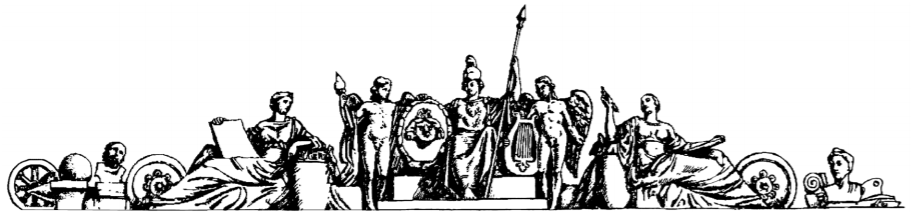
\includegraphics[scale=0.5]{hat.png}
\end{figure}

\begin{center}
МОСКОВСКИЙ ГОСУДАРСТВЕННЫЙ ТЕХНИЧЕСКИЙ
УНИВЕРСИТЕТ им. Н. Э. БАУМАНА \\
\end{center}

\vspace{6em}

\begin{center}
\Large Факультет «Робототехника и комплексная автоматизация» \\
\Large Кафедра «Системы автоматизированного проектирования» \\ 
\end{center}

\vspace{2em}

\begin{center}
\textsc{\textbf{Отчет по лабораторным работам по курсу
 \linebreak «Введение в искуственный интеллект»}}
\end{center}

\vspace{16em}



\newbox{\lbox}
\savebox{\lbox}{\hbox{Федорук В.Г.}}
\newlength{\maxl}
\setlength{\maxl}{\wd\lbox}
\hfill\parbox{11cm}{
\hspace*{5cm}\hspace*{-2cm}Студент:\hfill\hbox to\maxl{Задорожный В.В.\hfill}\\
\hspace*{5cm}\hspace*{-2cm}Преподаватель:\hfill\hbox to\maxl{Федорук В.Г.}\\
\hspace*{5cm}\hspace*{-2cm}Группа:\hfill\hbox to\maxl{РК6-11М}\\
}


\vspace{\fill}

\begin{center}
Москва \\2018
\end{center}

\end{titlepage}
% это титульный лист
\newpage
\tableofcontents % это оглавление, которое генерируется автоматически
\newpage
%\section{Лабораторная работа 2 (вариант 59)}
\subsection{Задание}


Ферзь находится на поле A1 шахматной доски. Необходимо найти замкнутый маршрут из 14 ходов, обеспечивающий прохождение всех полей доски. При этом любые поля допускается проходить более одного раза.

\subsection{Иходный код}
\begin{verbatim}
     1	gen_desk(_,0,[]):-!.
     2	gen_desk(0,J,D):- J>0, J1 is J - 1, gen_desk(8, J1, D),!.
     3	gen_desk(I,J,[c(I,J,n) | D]) :- I>0, I1 is I-1, gen_desk(I1, J, D). 
     4	
     5	direction([],1):-!.
     6	direction([1],3):-!.
     7	direction([I|_],I1):- I1 is (I+3) mod 8.
     8	
     9	isEnd([]):-!.
    10	isEnd([c(_,_,y)|Desk]):-isEnd(Desk).
    11	
    12	nCoord(X,Y,X1,Y1, 0):-X<8,Y>1,X1 is X+1, Y1 is Y - 1,!.
    13	nCoord(X,Y,X1,Y,1):-X<8,X1 is X+1,!.
    14	nCoord(X,Y,X1,Y1,2):-X<8,Y<8,X1 is X+1, Y1 is Y+1,!.
    15	nCoord(X,Y,X,Y1,3):-Y<8,Y1 is Y+1,!.
    16	nCoord(X,Y,X1, Y1,4):-X>1,Y<8,X1 is X-1, Y1 is Y+1,!.
    17	nCoord(X,Y,X1, Y,5):-X>1,X1 is X-1,!.
    18	nCoord(X,Y,X1, Y1, 6):-X>1,Y>1,X1 is X-1, Y1 is Y-1,!.
    19	nCoord(X,Y,X,Y1, 7):-Y>1,Y1 is Y-1,!.
    20	
    21	broken(1,1,[],_,Desk):-isEnd(Desk).
    22	broken(X,Y,[X1,Y1|Broken],Dir,Desk):-
    23	    direction(Dir,NDir),
    24	    line(X,Y,X1,Y1,NDir,Desk,Desk1,L),
    25		L>2,
    26		broken(X1,Y1,Broken,[NDir|Dir],Desk1).
    27	
    28	line(X,Y,X0,Y0,Dir,Desk,Desk0,IJ):-
    29		nCoord(X,Y,X1,Y1,Dir),
    30	    mark(X1,Y1,Desk,Desk1,J),
    31	    line(X1,Y1,X0,Y0,Dir,Desk1,Desk0,I),
    32		IJ is I + J.
    33	line(X,Y,X,Y,_,Desk,Desk,0).
    34	
    35	mark(X,Y,[c(X,Y,n)|Desk],[c(X,Y,y)|Desk],1):-!.
    36	mark(X,Y,[c(X,Y,y)|Desk],[c(X,Y,y)|Desk],0):-!.
    37	mark(X,Y,[Cell|Desk],[Cell|Desk1],I):-mark(X,Y,Desk,Desk1,I).
    38	
    39	run :-
    40		gen_desk(8,8,Desk),
    41		broken(1,1,Broken,[],Desk),
    42		format('Путь: ~w~n', [[1,1|Broken]]),
    43		fail;
    44		write('Готово.').gen_desk(_,0,[]):-!.
    45		gen_desk(0,J,D):- J>0, J1 is J - 1, gen_desk(8, J1, D),!.
    46		gen_desk(I,J,[c(I,J,n) | D]) :- I>0, I1 is I-1, gen_desk(I1, J, D). 
\end{verbatim}
\subsection{Результат}
\begin{verbatim}
    ?- [ferz].
    true.

    ?- run
    |    .
    Путь: [1,1,8,1,8,8,2,2,8,2,2,8,2,4,6,8,3,8,7,4,7,8,2,3,6,3,1,8,1,1]
    Путь: [1,1,8,1,8,8,3,3,7,3,2,8,2,4,6,8,3,8,7,4,7,8,1,2,7,2,1,8,1,1]
    Готово.
    true.
\end{verbatim}

Получено два варинта маршрута:

\begin{figure}[H]
\centering
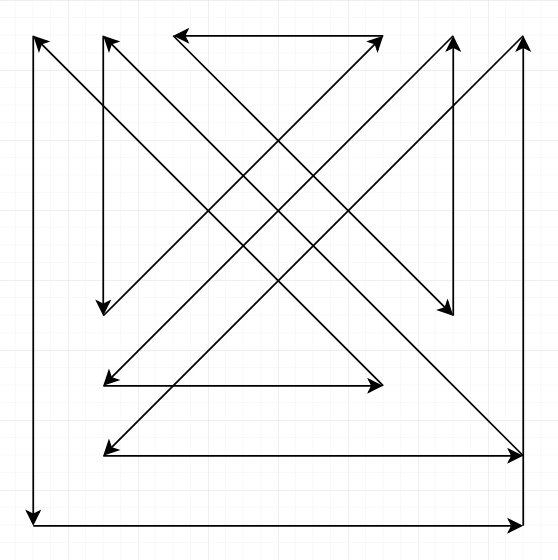
\includegraphics[scale=0.5]{way1.jpeg}
\caption{Маршрут 1}
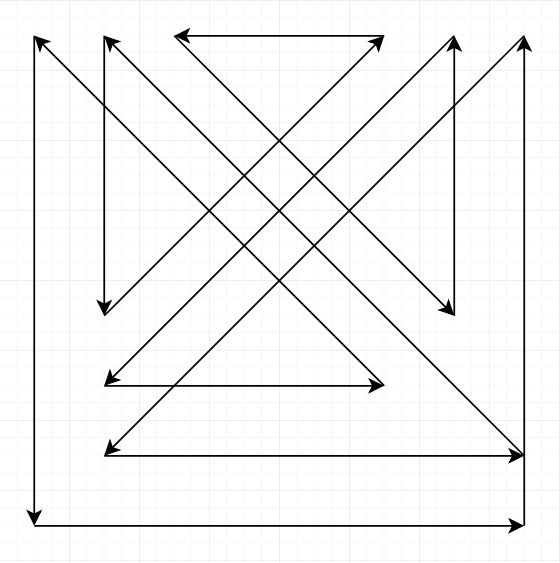
\includegraphics[scale=0.51]{way2.jpeg}
\caption{Маршрут 2}
\label{img:ways}
\end{figure}

%\section{Лабораторная работа 3 (вариант 5-8)}

\subsection{Задание}
Цель работы - создание программы, реализующей искусственный нейрон; разработка процедуры обучения нейрона; использование полученных результатов для решения тестовых задач классификации и аппроксимации.

\subsection{WTA нейрон}
Нейроны типа WTA (Winner Takes All — победитель получает все) всегда используются группами, в которых конкурируют между собой. Структурная схема группы (слоя) нейронов типа WTA представлена на рисунке ниже (рисунок \ref{img:wta}).

\begin{figure}[H]
\centering
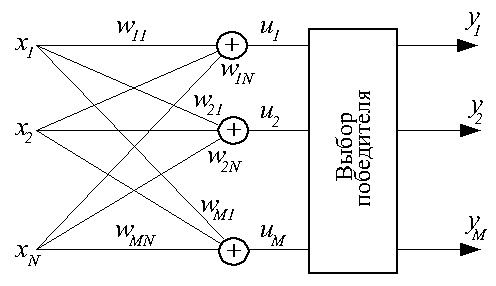
\includegraphics[scale=0.5]{wta.png}
\caption{Структурная схема слоя нейрона типа WTA}
\label{img:wta}
\end{figure}

Каждый конкурирующий нейрон в группе получает одни и те же входные сигналы. Каждый нейрон рассчитывает выходной сигнал своего сумматора обычным образом:

\begin{equation}\label{eq:Func}
	u_i=\sum\limits_{j=0}^N w_{ij} x_j.
\end{equation}

\begin{itemize}
\item По результатам сравнения всех $u_i, j=1, 2, ..., M$ выбирается нейрон-победитель, обладающий наибольшим значением $u_i$. Выходной сигнал $y_i$ нейрона-победителя получает значение 1, выходные сигналы всех остальных нейронов — 0.
\end{itemize}

Для обучения нейронов типа WTA не требуется учитель, оно практически полностью аналогично обучению инстара Гроссберга. Начальные значения весовых коэффициентов всех нейронов выбираются случайным образом с последующей нормализацией относительно 1.
При предъявлении каждого обучающего вектора $X^k$ определяется нейрон-победитель, что дает ему право уточнить свои весовые коэффициенты по упрощенному (в силу бинарности $y_i$) правилу Гроссберга:

\begin{equation}\label{eq:Func}
    w_{ij}(t+1)=w_{ij}(t)+\eta(x_j^k-w_{ij}(t)).
\end{equation}
Все проигравшие нейроны оставляют свои весовые коэффициенты неизменными. 

В каждом цикле обучения побеждает тот нейрон, чей текущий вектор входных весов $W_i$ наиболее близок входному вектору $X_k$. При этом вектор $W_i$ корректируется в сторону вектора $X_k$. Поэтому в ходе обучения каждая группа близких друг другу входных векторов (кластер) обслуживается отдельным нейроном.




Понятие «близости» двух векторов можно продемонстрировать на следующем примере. Пусть на очередной итерации обучения сети в режиме «онлайн» имеется входной вектор $X^k$. Тогда вычисление взвешенной суммы для i-го нейрона осуществляется по формуле:
\begin{equation}\label{eq:sum_func}
    u _ { i } = W _ { i } ^ { T } \cdot X ^ { k } = \sum _ { j = 1 } ^ { N } w _ { i j } \cdot x _ { j } ^ { k } = \left\| W _ { i } ^ { T } \right\| \cdot \left\| X ^ { k } \right\| \cdot \cos \left( \sphericalangle   W _ { i } , X ^ { k } \right)
\end{equation}

Поскольку вектора $W_i$ и $X^k$ нормализованы, то взвешенная сумма i-го нейрона равна косинусу угла между вектором весов и входным вектором. На рис. \ref{img:angle} представлена геометрическая интерпретация. Чем ближе весовой вектор ко входному, тем ближе косинус угла между векторами к 1.

\begin{figure}[H]
\centering
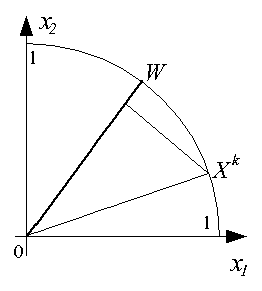
\includegraphics[scale=0.5]{angle.png}
\caption{Геометрическая интерпретация весов нейронов}
\label{img:angle}
\end{figure}

В режиме кластеризации при подаче на вход слоя нейронов типа WTA очередного вектора $X^k$ определяется степень его близости к векторам $W_i$ в виде косинусов углов между этими векторами, после чего определяется наиболее «близкий» вектор весов, отвечающий за тот или иной кластер.

Результат обучения слоя нейронов типа WTA на последовательности девяти двухкомпонентных входных векторов ${X^1, X^2, ..., X^9}$ иллюстрирует (рис. \ref{img:wta_teached}). Здесь были выделены три кластера входных векторов $\{X^1, X^8\}$, $\{X^3, X^4, X^5\}$ и $\{X^2, X^6, X^7, X^9\}$. За их распознавание отвечают три нейрона с векторами входных весов $W_1$, $W_2$ и $W_3$ соответственно.

\begin{figure}[H]
\centering
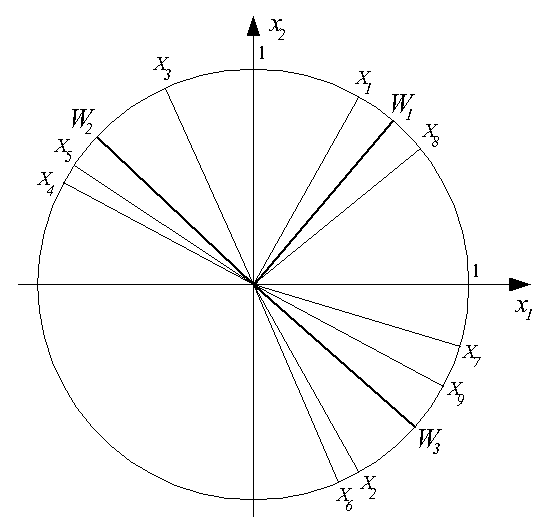
\includegraphics[scale=0.4]{wta_teached.png}
\caption{Результат обучения слоя нейронов типа WTA}
\label{img:wta_teached}
\end{figure}

Серьезная проблема в использовании нейронов типа WTA — возможность возникновения "мертвых" нейронов, т.е. нейронов, ни разу не победивших в конкурентной борьбе в ходе обучения и поэтому оставшихся в начальном состоянии. Для исключения "ложных" срабатываний в режиме классификации мертвые нейроны после окончания обучения должны быть удалены.

Для уменьшения количества мертвых нейронов (и, следовательно, повышения точности распознавания) используется модифицированное обучение, основанное на учете числа побед нейронов и шрафовании наиболее "зарвавшихся" среди них. Дисквалификация может быть реализована либо назначением порога числа побед, после которого слишком активный нейрон "засыпает" на заданное число циклов обучения, либо искусственным уменьшением величины  пропорционально числу побед.



\subsection{Исходные данные}

Обучающие данные для варианта 8 представлены на рисунке \ref{img:train_sphere}.

\begin{figure}[H]
\centering
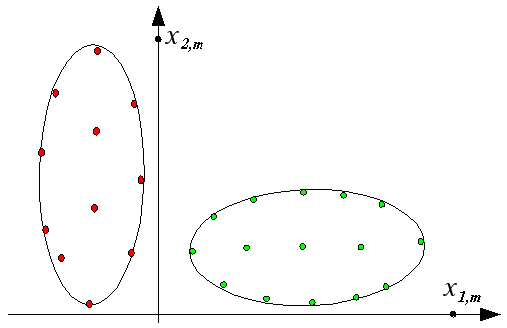
\includegraphics[scale=0.6]{train_sphere.png}
\caption{Данные для обучения варианта 8}
\label{img:train_sphere}
\end{figure}

\subsection{Обучение}

Для обучения были сгенерированы в случайном порядке точки, принадлежашие двум областям (рис. \ref{img:points}, а). После этого вектор входных значений, состоящих из координат точек, был нормализован (рис. \ref{img:points}, б) по формуле:
\begin{equation}\label{eq:normaFunc}
	x_{j}\leftarrow\frac{x_{j}}{\sqrt{x_{1}^{2}+x_{2}^{2}+\ldots+x_{N}^{2}}}.
\end{equation}

%\begin{figure}[h]
%    \begin{center}
%        \begin{minipage}[h]{0.48\linewidth}
%            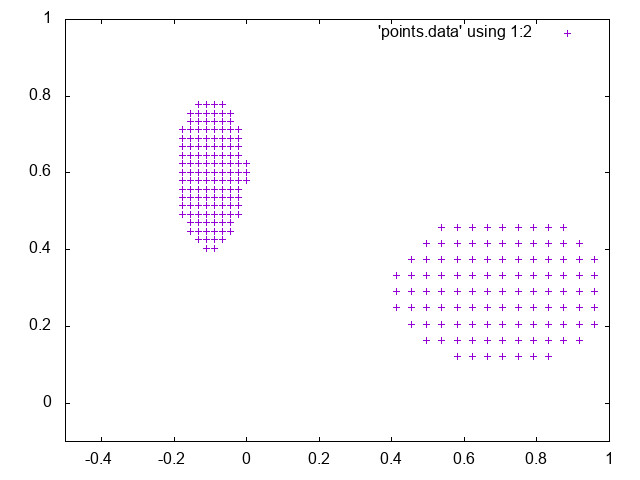
\includegraphics[width=1\linewidth]{points_nonorma.jpg}
%            %\caption{Обучающие данные} %% подпись к рисунку
%            \label{img:points} %% метка рисунка для ссылки на него
%        \end{minipage}
%        \hfill 
%        \begin{minipage}[h]{0.48\linewidth}
%            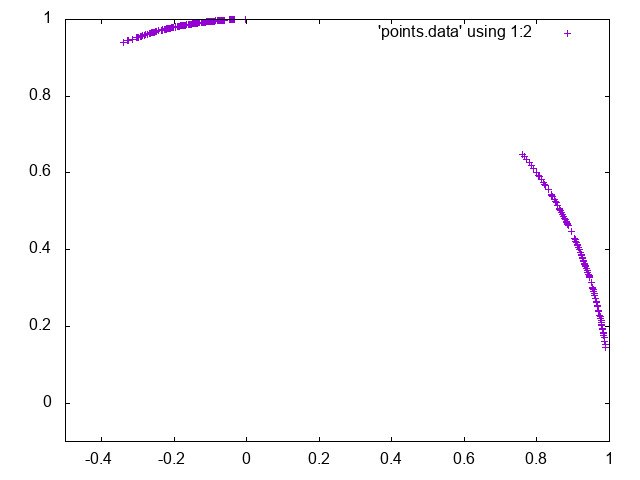
\includegraphics[width=1\linewidth]{points.png}
%            %\caption{Обчающие данные нормализованные}
%            \label{img:points_norma}
%        \end{minipage}
%        \begin{minipage}[h]{1\linewidth}
%            \centering
%            \begin{tabular}{p{0.50\linewidth}p{0.40\linewidth}}
%                %\centering % Обчающие данные после нормализации &
%                    \caption{Обучающие данные} &
%                %\centering %Обчающие данные после нормализации \\
%                    \caption{Обчающие данные после нормализации} \\
%            \end{tabular}
%        \end{minipage}
%    \end{center}
%\end{figure}


\begin{figure}[h]
    \begin{minipage}[h]{0.49\linewidth}
        \center{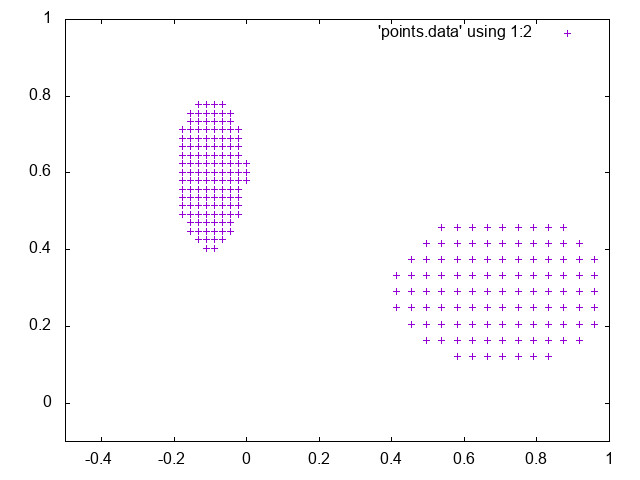
\includegraphics[width=1\linewidth]{points_nonorma.jpg} \\ а)}
    \end{minipage}
    \hfill
    \begin{minipage}[h]{0.49\linewidth}
        \center{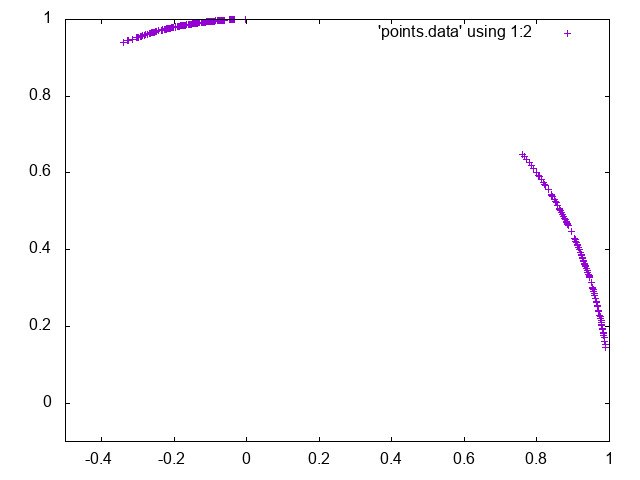
\includegraphics[width=1\linewidth]{points.png} \\ б)}
    \end{minipage}
    \caption{Обучающие данные}
    \label{img:points}
\end{figure}


Оба множнста имеют примерно одинаковое количесво точек. Это сделано, чтобы не допусть паревеса весов в сторону какого-либо из множеств.

Параметры обучения:
\begin{itemize}
    \item Размерность входных векторов: 2
    \item Количество нейронов: 4
    \item Количество эпох обучения: 2
    \item Коэффициент обучения $\eta$: 0,1
    \item Коэффициент штрафа при обучении: 0,01
    \item Начальные значения весов: (-1, -1) для всех весов
\end{itemize}

Обучение проводилось онлайн-методом - корректировка весов проводилась после подачи каджого входного вектора.

Коэффициент штрафа при обучении необходим для решения проблемы «мертвых» нейронов. Для каждого нейрона в слое вводится счетчик побед. Он изменяется на каждой итерации обучения для нейронов-победителей. Считчик используется для коррекции взвешенных сумм нейронов перед процедурой определения нейрона-победителя. Взвешенная сумма каждого нейрона рассчитывается по формуле:
\begin{equation}\label{eq:penaltyFunc}
    u _ { i } = \left( \sum _ { j = 1 } ^ { N } w _ { i j } \cdot x _ { j } \right) - p \cdot C_i,
\end{equation}
где $C_i, i=1, 2, ..., M$ - счетчик побед, p - коэффициент штрафа при обучении.

\subsection{Результат}

Результат процесса обучения представлен на рис. \ref{img:result}

\begin{figure}[h]
    \begin{minipage}[h]{0.49\linewidth}
        \center{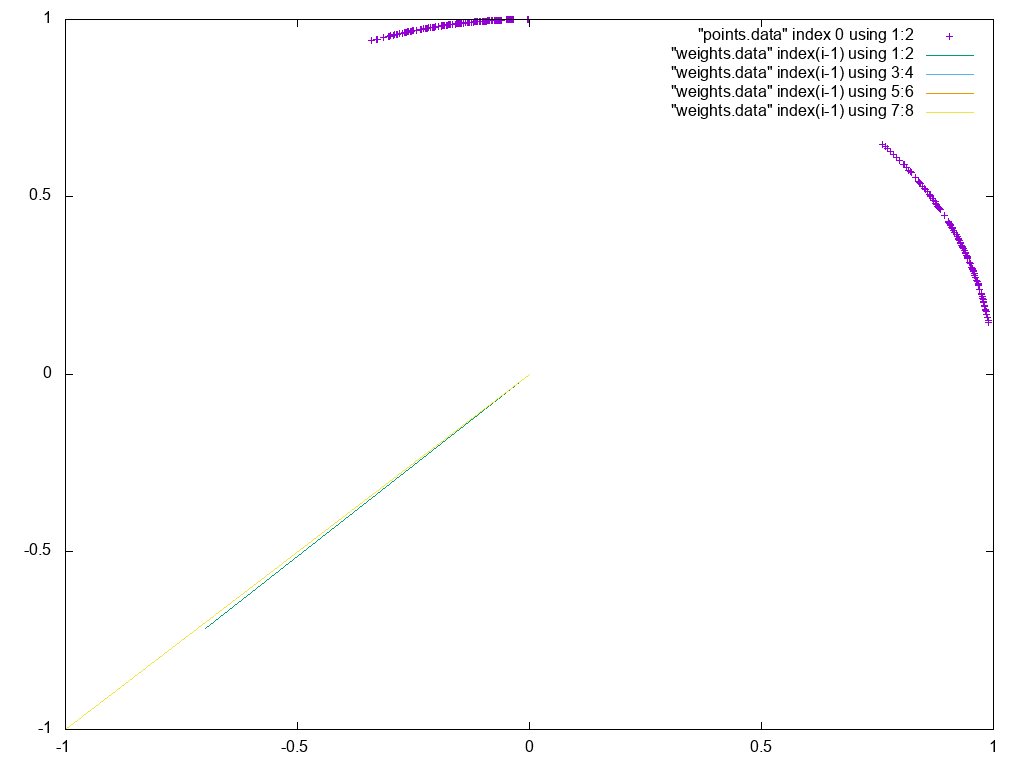
\includegraphics[width=1\linewidth]{train0.png} \\ а)}
    \end{minipage}
    \hfill
    \begin{minipage}[h]{0.49\linewidth}
        \center{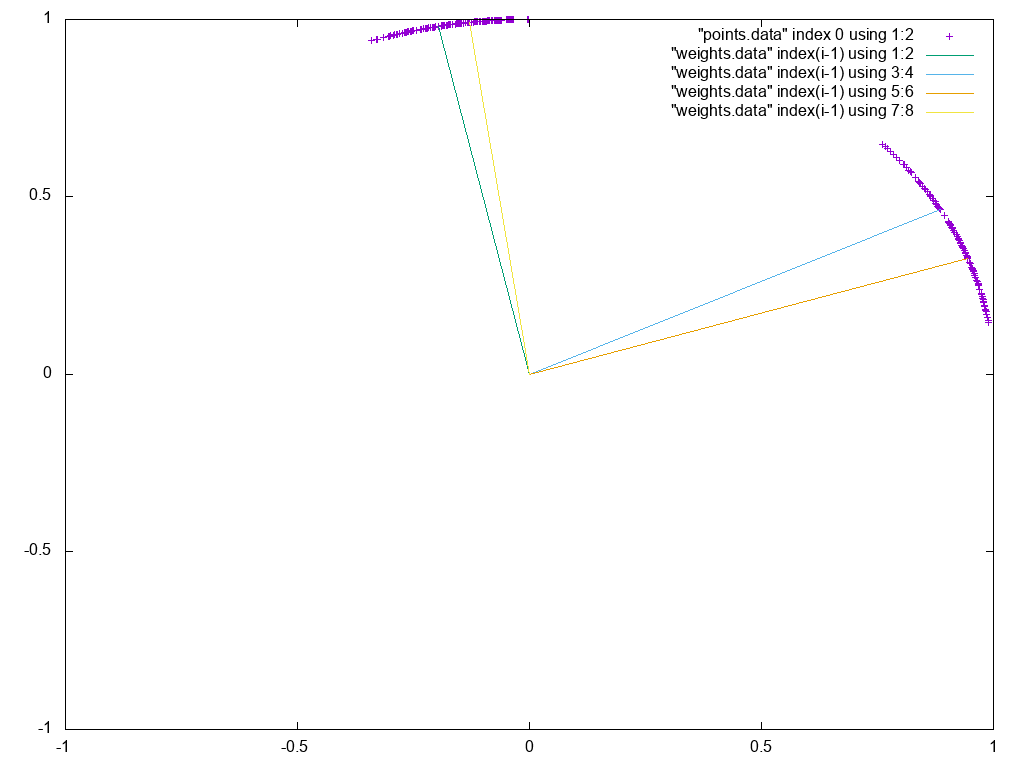
\includegraphics[width=1\linewidth]{train6.png} \\ б)}
    \end{minipage}
    \caption{a) - нулевое положение, б) - конечный результат}
    \label{img:result}
\end{figure}

Сам процесс обучения частично предствлен на рис. \ref{img:teaching}. Из начального положения $(x_1, x_2) = (-1, -1)$ (рис.\ref{img:teaching}, a), значения весов векторов  постепенно выравниваются и достигаю конечнго распределения, как на (рис.\ref{img:result}).

\begin{figure}[H]
    \begin{minipage}[h]{0.47\linewidth}
        \center{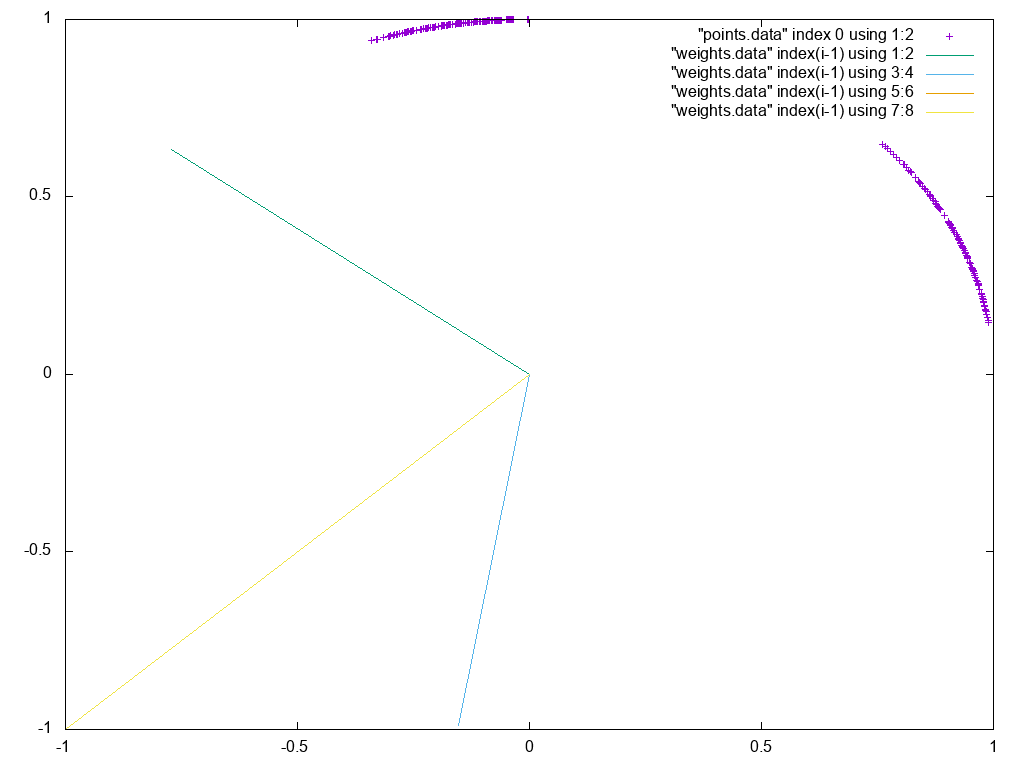
\includegraphics[width=1\linewidth]{train1.png} а)}  \\
    \end{minipage}
    \hfill
    \begin{minipage}[h]{0.47\linewidth}
        \center{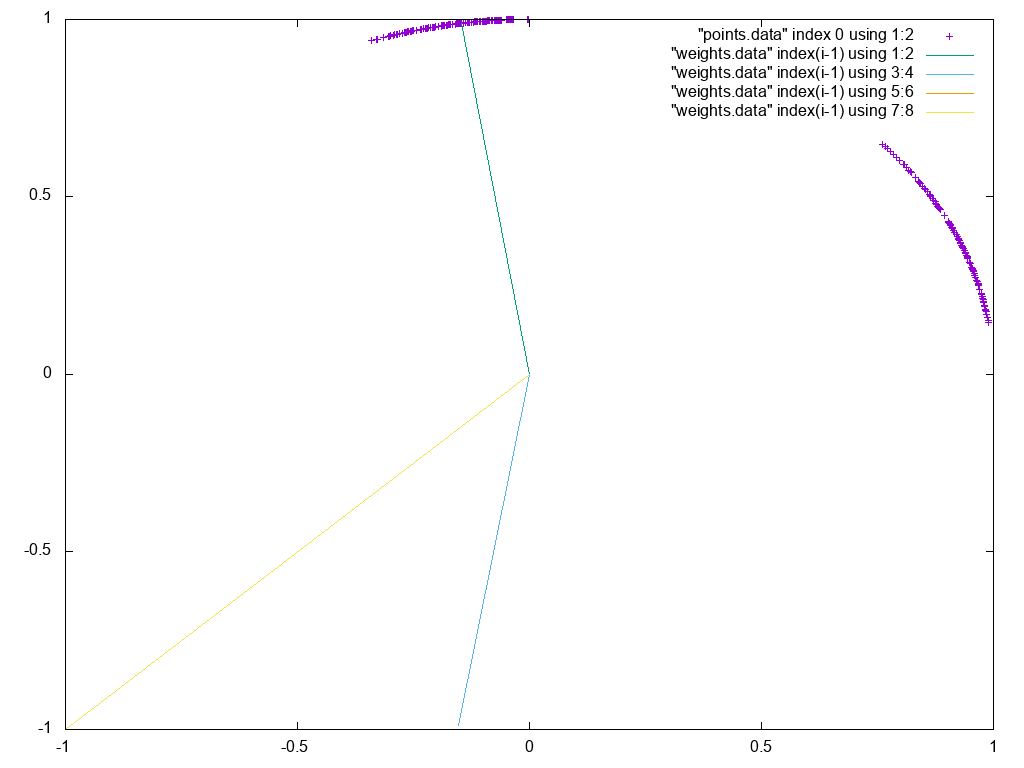
\includegraphics[width=1\linewidth]{train11.png} б)} \\
    \end{minipage}
    \vfill
    \begin{minipage}[h]{0.47\linewidth}
        \center{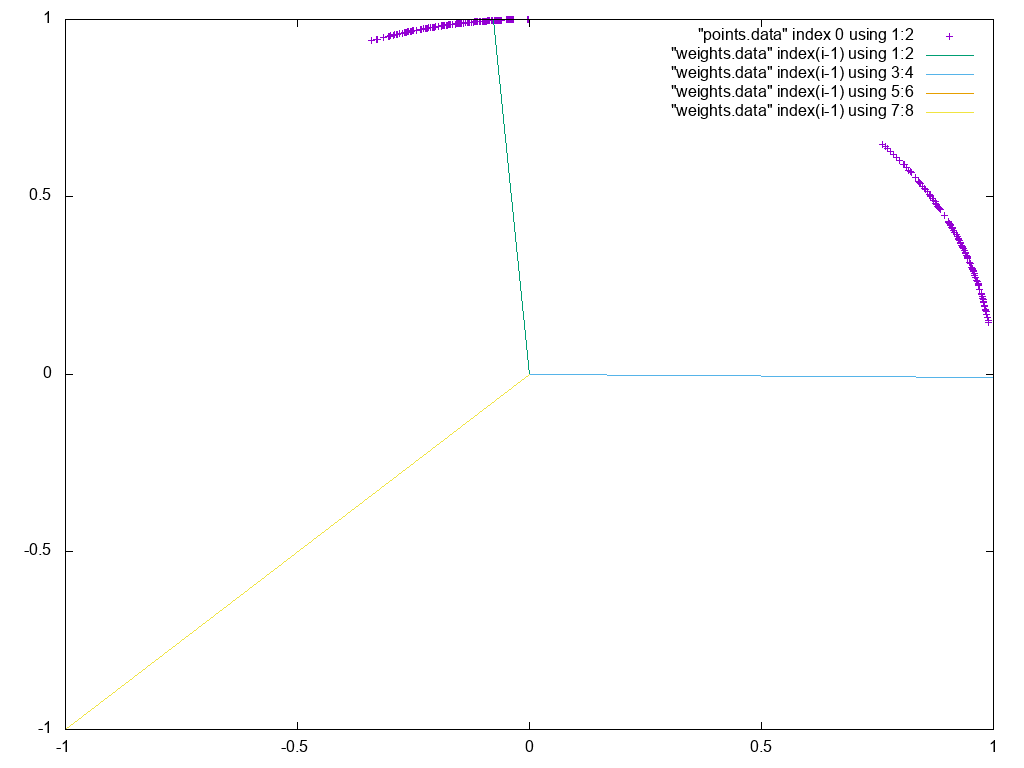
\includegraphics[width=1\linewidth]{train2.png} в)} \\
    \end{minipage}
    \hfill
    \begin{minipage}[h]{0.47\linewidth}
        \center{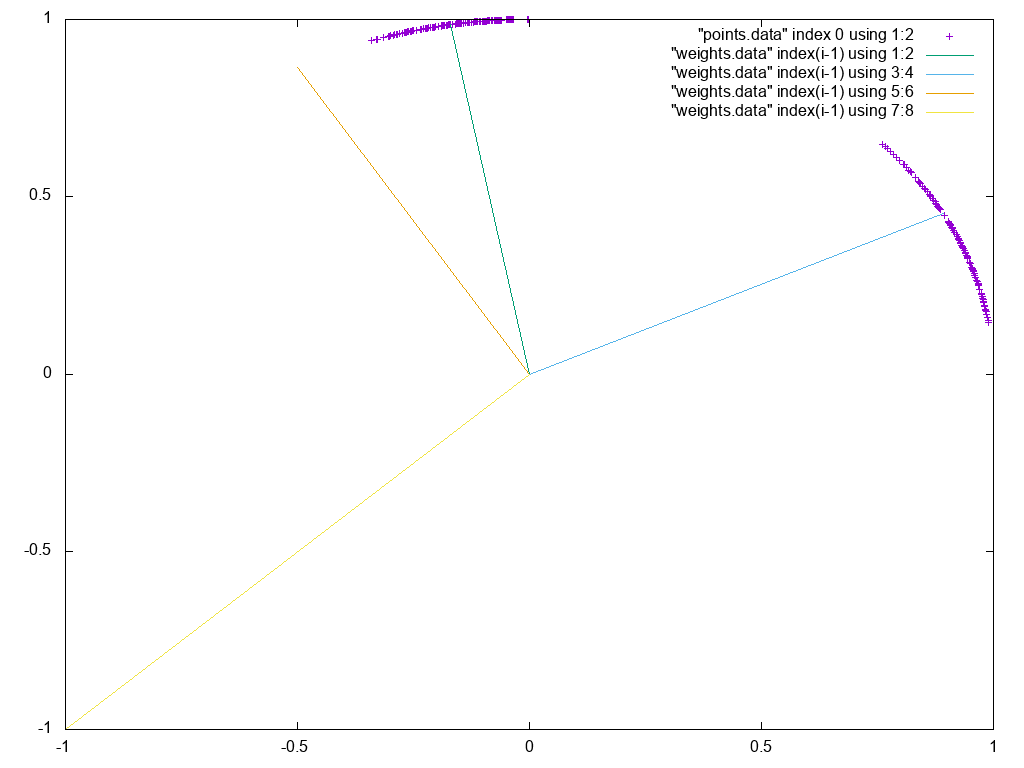
\includegraphics[width=1\linewidth]{train3.png} г)} \\
    \end{minipage}
    \vfill
    \begin{minipage}[h]{0.47\linewidth}
        \center{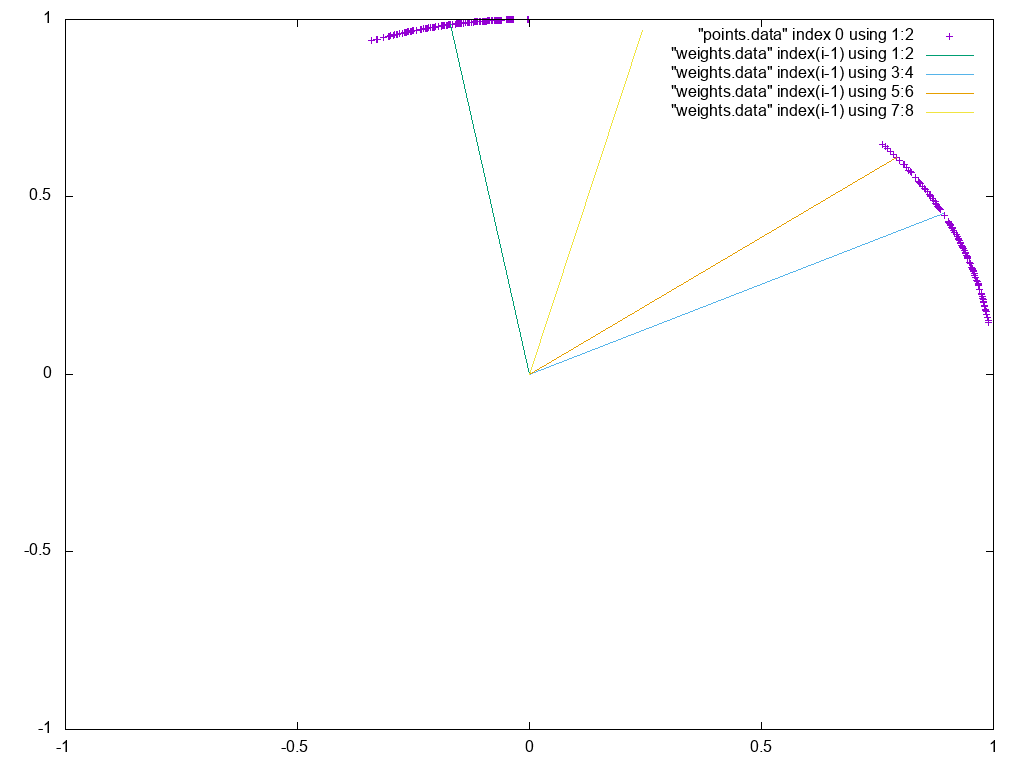
\includegraphics[width=1\linewidth]{train4.png} д)}  \\
    \end{minipage}
    \hfill
    \begin{minipage}[h]{0.47\linewidth}
        \center{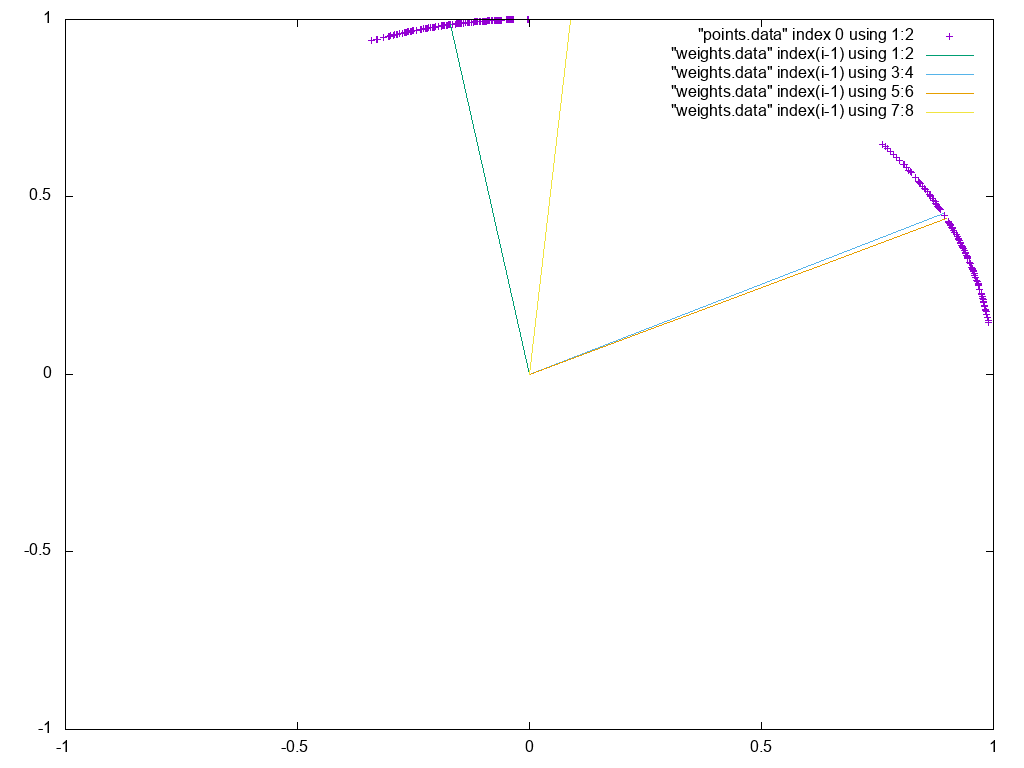
\includegraphics[width=1\linewidth]{train5.png} е)} \\
    \end{minipage}
    \caption{Процесс обучения}
    \label{img:teaching}
\end{figure}


\subsection{Иходный код}
Файл main.cpp
\begin{verbatim}
     1	#include "WTA.h"
     2	#include <algorithm>
     3	#include <cmath>
     4	
     5	void GenerateElipsis2DPointSet(
     6	        std::vector<std::vector<double>> *points,
     7	        double a, double b,
     8	        double xOffset, double yOffset,
     9	        double rotation, double step) {
    10	    a = (a < 0) ? -a : a;
    11	    b = (b < 0) ? -b : b;
    12	    double norm;
    13	
    14	    for (double x = -a; x <= a; x += step) {
    15	        for (double y = -b; y <= b; y += step) {
    16	            if (((x * x) / (a * a) + (y * y) / (b * b)) <= 1) {
    17	                std::vector<double> v(2);
    18	                v[0] = (x * cos(rotation) + y * sin(rotation)) + xOffset
;
    19	                v[1] = (-x * sin(rotation) + y * cos(rotation)) + yOffse
t;
    20	                norm = sqrt(v[0] * v[0] + v[1] * v[1]);
    21	                // normalize
    22	                v[0] /= norm;
    23	                v[1] /= norm;
    24	                points->emplace_back(std::move(v));
    25	            }
    26	        }
    27	    }
    28	
    29	    std::cout << "finish" << std::endl;
    30	}
    31	
    32	std::vector<std::vector<double>> Generate2DTrainSet() {
    33	    std::vector<std::vector<double>> trainSet;
    34	
    35	    GenerateElipsis2DPointSet(&trainSet, 0.3, 0.2, 0.7, 0.3, -M_PI, 0.04
2);
    36	    GenerateElipsis2DPointSet(&trainSet, 0.2, 0.1, -0.1, 0.6, M_PI_2, 0.
022);
    37	
    38	    std::random_shuffle(trainSet.begin(), trainSet.end());
    39	    return trainSet;
    40	}
    41	
    42	void DumpPoints(std::ostream &output, const std::vector<std::vector<doub
le>> &points) {
    43	    for (size_t iPoint = 0; iPoint < points.size(); ++iPoint) {
    44	        for (size_t iCoord = 0; iCoord < points[iPoint].size(); ++iCoord
)
    45	            output << points[iPoint][iCoord] << "\t";
    46	
    47	        output << std::endl;
    48	    }
    49	}
    50	
    51	int main() {
    52	    const std::string WEIGHTS_DUMP_FILE = "weights.data";
    53	    const std::string TRAIN_SET_FILE    = "points.data";
    54	    
    55	    WTALayer nnet;
    56	    WTALayer::Config nnetConfig;
    57	
    58	    nnetConfig.neurons  = 4;
    59	    nnetConfig.inVecDim = 2;
    60	    nnetConfig.trainEpochs = 2;
    61	    nnetConfig.trainCoeff  = 0.1;
    62	    nnetConfig.trainPenalty = 0.01;
    63	    const std::vector<double> INITIAL_WEIGHTS(nnetConfig.neurons * nnetC
onfig.inVecDim, -1.0);
    64	
    65	    nnet.Init(nnetConfig, false);
    66	
    67	    if (!nnet.SetWeights(INITIAL_WEIGHTS))
    68	        return 1;
    69	
    70	    nnet.DumpWeights(std::cout, 6, "Initial weights:");
    71	    std::ofstream trainSetDump(TRAIN_SET_FILE, std::ios::binary);
    72	    std::ofstream weightsDump(WEIGHTS_DUMP_FILE, std::ios::binary);
    73	    std::vector<std::vector<double>> trainSet(std::move(Generate2DTrainS
et()));
    74	    DumpPoints(trainSetDump, trainSet);
    75	    nnet.Train(trainSet, weightsDump);
    76	    nnet.DumpWeights(std::cout, 6, "Result weights:");
    77	}
\end{verbatim}

Файл WTA.h
\begin{verbatim}
     1	#ifndef LAB3_WTA_LAYER_H
     2	#define LAB3_WTA_LAYER_H
     3	
     4	#include <vector>
     5	#include <iostream>
     6	#include <fstream>
     7	using size_t = std::size_t;
     8	
     9	class WTALayer {
    10	public:
    11	    struct Config {
    12	        size_t neurons;
    13	        size_t inVecDim;
    14	        int    trainEpochs;
    15	        double trainCoeff;
    16	        double trainPenalty;
    17	    };
    18	
    19	    void Init(const Config &conf, bool randomizeWeights = true);
    20	    bool SetWeights(const std::vector<double> &initialWeights);
    21	    size_t Test(const std::vector<double> &inVec);
    22	
    23	    void Train(const std::vector<std::vector<double>> &trainSet,
    24	        std::ostream &output);
    25	
    26	    void DumpWeights(std::ostream &output, int precision,
    27	        const std::string &title = "", bool gnuplot = false);
    28	
    29	private:
    30	    Config config;
    31	    std::vector<double>   weights;
    32	    std::vector<uint64_t> winHistory;
    33	
    34	    void RandomizeWeights();
    35	    std::vector<double> GetWeightedSums(const std::vector<double> &inVec;
    36	    size_t DetectWinner(const std::vector<double> &weightedSums);
    37	    void AdjustWeights(size_t iWinner, const std::vector<double> &inVec);
    38	
    39	    void AdjustWinHistory(size_t iWinner) { winHistory[iWinner] += 1; }
    40	};
    41	
    42	#endif
\end{verbatim}

Файл WTA.cpp
\begin{verbatim}
     1	#include "WTA.h"
     2	#include <iomanip>
     3	#include <random>
     4	#include <algorithm>
     5	
     6	void WTALayer::Init(const Config &conf, bool randomizeWeights) {
     7	    config = conf;
     8	
     9	    if (!randomizeWeights)
    10	        return;
    11	
    12	    weights.resize(config.neurons * config.inVecDim);
    13	    winHistory.resize(config.neurons * config.inVecDim, 0);
    14	    RandomizeWeights();
    15	}
    16	
    17	bool WTALayer::SetWeights(const std::vector<double> &initialWeights) {
    18	    if (initialWeights.size() != config.neurons * config.inVecDim) {
    19	        std::cerr << "invalid weights size: " << initialWeights.size() <
< std::endl;
    20	        return false;
    21	    }
    22	
    23	    weights = initialWeights;
    24	    winHistory.resize(config.neurons * config.inVecDim, 0);
    25	
    26	    return true;
    27	}
    28	
    29	void WTALayer::RandomizeWeights() {
    30	    const double WEIGHT_INF = 1.0;
    31	    const double WEIGHT_SUP = -1.0;
    32	
    33	    std::random_device randomizer;
    34	    std::mt19937 randGen(randomizer());
    35	    std::uniform_real_distribution<> dist(WEIGHT_INF, WEIGHT_SUP);
    36	
    37	    double weightNorm;
    38	    double weight = 0.0;
    39	
    40	    // randomize and normalize all weights
    41	    for (size_t iNeuron = 0; iNeuron < config.neurons; ++iNeuron) {
    42	        weightNorm = 0.0;
    43	
    44	        for (size_t iWeight = 0; iWeight < config.inVecDim; ++iWeight) {
    45	            weight = dist(randGen);
    46	            weights[iWeight + iNeuron * config.inVecDim] = weight;
    47	            weightNorm += weight * weight;
    48	        }
    49	
    50	        weightNorm = sqrt(weightNorm);
    51	
    52	        for (size_t iWeight = 0; iWeight < config.inVecDim; ++iWeight)
    53	            weights[iWeight + iNeuron * config.inVecDim] /= weightNorm;
    54	    }
    55	}
    56	
    57	std::vector<double> WTALayer::GetWeightedSums(const std::vector<double> 
&inVec) {
    58	    std::vector<double> weightedSums(config.neurons, 0.0);
    59	    
    60	    for (size_t iNeuron = 0; iNeuron < config.neurons; ++iNeuron) {
    61	        for (size_t iWeight = 0; iWeight < config.inVecDim; ++iWeight) {
    62	            weightedSums[iNeuron] += weights[iWeight + iNeuron * config.
inVecDim] * inVec[iWeight];
    63	            // TODO code refactoring
    64	            weightedSums[iNeuron] -= config.trainPenalty * winHistory[iN
euron];
    65	        }
    66	    }
    67	    for (double &a : weights)
    68	        std::cout << a << ' ';
    69	    std::cout << std::endl;
    70	    return weightedSums;
    71	}
    72	
    73	size_t WTALayer::DetectWinner(const std::vector<double> &weightedSums) {
    74	    return std::distance(weightedSums.begin(),
    75	        std::max_element(weightedSums.begin(), weightedSums.end()));
    76	}
    77	
    78	size_t WTALayer::Test(const std::vector<double> &inVec) {
    79	    if (inVec.size() != config.inVecDim)
    80	        throw std::string("WTALayer::Test --> invalid input vector size!
");
    81	
    82	    return DetectWinner(GetWeightedSums(inVec));
    83	}
    84	
    85	void WTALayer::AdjustWeights(size_t iWinner, const std::vector<double> &
inVec) {
    86	    double prevWeight;
    87	    double currWeight;
    88	    double weightNorm = 0.0;
    89	
    90	    for (size_t iWeight = 0; iWeight < config.inVecDim; ++iWeight) {
    91	        prevWeight = weights[iWeight + iWinner * config.inVecDim];
    92	        currWeight = prevWeight + config.trainCoeff * (inVec[iWeight] - 
prevWeight);
    93	        weights[iWeight + iWinner * config.inVecDim] = currWeight;
    94	        weightNorm += currWeight * currWeight;
    95	    }
    96	
    97	    weightNorm = sqrt(weightNorm);
    98	
    99	    // normalize weights
   100	    for (size_t iWeight = 0; iWeight < config.inVecDim; ++iWeight) {
   101	        weights[iWeight + iWinner * config.inVecDim] /= weightNorm;
   102	    }
   103	}
   104	
   105	void WTALayer::Train(const std::vector<std::vector<double>> &trainSet, s
td::ostream &output) {
   106	    size_t iWinner;
   107	
   108	    for (size_t iEpoch = 0; iEpoch < config.trainEpochs; ++iEpoch) {
   109	        std::cout << "Train epoch: " << iEpoch << std::endl;
   110	
   111	        for (size_t iVec = 0; iVec < trainSet.size(); ++iVec) {
   112	            iWinner = Test(trainSet[iVec]);
   113	            AdjustWinHistory(iWinner);
   114	            std::cout << "Победитель" << iWinner << std::endl;
   115	            AdjustWeights(iWinner, trainSet[iVec]);
   116	
   117	            DumpWeights(output, 16, "", true);
   118	        }
   119	    }
   120	}
   121	
   122	void WTALayer::DumpWeights(std::ostream &output, int precision,
   123	        const std::string &title, bool gnuplot) {
   124	    if (!gnuplot)
   125	        output << title << std::endl;
   126	
   127	    if (gnuplot) {
   128	        for (size_t iWeight = 0; iWeight < weights.size(); ++iWeight)
   129	            output << 0.0 << "\t";
   130	
   131	        output << std::endl;
   132	    }
   133	
   134	    for (size_t iWeight = 0; iWeight < weights.size(); ++iWeight)
   135	        output << std::setprecision(precision) << weights[iWeight] << "\
t";
   136	
   137	    output << std::endl;
   138	
   139	    if (gnuplot)
   140	        output << std::endl << std::endl;
   141	}
\end{verbatim}

%\newpage
\section{Лабораторная работа 4 (Вариант 4)}
\subsection{Задание}

Выполнить классификацию двухмерных данных при помощи сети с самоорганизацией на основе конкуренции, обучающейся по алгоритму нейронного газа.

\subsection{Описание сетей с самоорганизацией на основе конкуренции}
Сетями с самоорганизацией называются сети, не требующие для своего
обучения «учителя» и самостоятельно адаптирующие свои веса под обучающие
данные. Такие сети строятся из нейронов типа WTA и подобных
им. Как правило, это однослойные сети, в которых каждый нейрон получает
все компоненты входного вектора $X$ размерностью $N$. На рисунке \ref{img:schemeNet_lab3}
представлена структурная схема такой сети.

\begin{figure}[H]
\centering
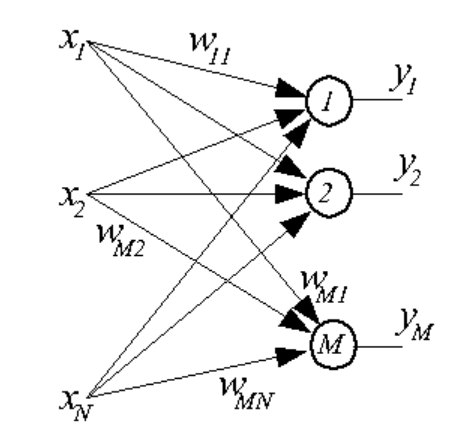
\includegraphics[scale=0.5]{schemeNet_lab3.png}
\caption{Схема сети с самоорганизацией на основе конкуренции}
\label{img:schemeNet_lab3}
\end{figure}

Веса входных связей $i$-ого нейрона образуют вектор
\begin{equation}
    W_{i} = \left[ \begin{array} { l l l l }{w_{i 1}} & {w_{i 2}}&{\dots}&{w_{ i N }}\end{array}\right]^{T} .
\end{equation}

Кроме связей, явно представленных в схеме, на этапе обучения имеют место
связи между нейронами, позволяющие судить о степени «соседства»
нейронов друг с другом, при этом смысл понятия «соседство» может
быть разным.
Укрупненно процесс обучения сети выглядит следующим образом. На
вход сети подается обучающий вектор $X^k$, для каждого нейрона определяется
$d(X^k, W_i)$ — расстояние (в смысле выбранной метрики) между
векторами $X_k$ и $W_i$. Определяется нейрон–победитель, для которого это
расстояние оказывается наименьшим. Вокруг нейрона–победителя образуется окрестность $S^k_w$ из нейронов–соседей с известным «расстоянием» до победителя. Веса нейрона–победителя и веса его соседей из $S^k_w$ уточняются, например, по правилу Кохонена:

\begin{equation}
	W_{i}^{k+1} = W_{i}^{k}+\eta_{i}^{k}\left(X^{k}-W_{i}^{k}\right) ,
\end{equation}

где $\eta^k_i$ --- коэффициент обучения, значение которого уменьшается с увеличением расстояния от $i$-ого нейрона до победителя. Веса нейронов вне $S^k_w$ не изменяются. Размер окрестности $S^k_w$ и величина $\eta^k_i$ с течением времени обучения уменьшаются.

В качестве меры измерения расстояния между векторами чаще всего
используются:

\begin{itemize}
\item евклидова мера $d \left( X , W _ { i } \right) = \left\| X - W _ { i } \right\| = \sqrt { \sum _ { j = 1 } ^ { N } \left( x _ { j } - w _ { i j } \right) ^ { 2 } }$
\item скалярное произведение
$d \left( X , W _ { i } \right) = 1 - X \cdot W _ { i } = 1 - \| X \| _ { 2 } \cdot \left\| W _ { i } \right\| _ { 2 } \cdot \cos \left( \angle X W _ { i } \right)$

\item манхэттеновское расстояние $d \left( X , W _ { i } \right) = \sum _ { j = 1 } ^ { N } \left| x _ { j } - w _ { i j } \right|$;

\item m-норма $d \left( X , W _ { i } \right) = \max _ { j } \left| x _ { j } - w _ { i j } \right|$.
\end{itemize}

\subsection{Проблема мертвых нейронов}
\label{seq:deadNeurons}
При «слепом» (как правило, случайном) выборе начальных значений весов
часть нейронов может оказаться в области пространства, в которой
отсутствуют обучающие данные или где их количество ничтожно мало.
Такие нейроны имеют очень мало шансов на победу в конкурентной
борьбе и адаптацию своих весов, вследствие чего они остаются мертвыми.
В итоге уменьшается количество активных нейронов, участвующих
в анализе входных данных, и, следовательно, увеличивается погрешность
их интерпретации, называемая погрешностью квантования. Встает проблема
активации всех нейронов сети на этапе обучения.
Такую активацию можно осуществить, базируясь на учете количества
побед, одержанных каждым нейроном в ходе обучения. Существуют
разные механизмы такого учета.
В одном из таких подходов каждому нейрону сети приписывается
потенциал $\pi_i$
, значение которого модифицируется после предъявления
каждого обучающего вектора $X^k$ по следующей формуле (в ней $w$ —
индекс нейрона-победителя):

\begin{equation}\label{eq:system}
		\begin{aligned}
		&	\pi _ { i } ^ { k + 1 } = \pi _ { i } ^ { k } + 1 / M, где i \neq w\\
		&   \pi _ { i } ^ { k + 1 } = \pi _ { i } ^ { k } - \pi _ { min }, где i = w.
		\end{aligned}  		
\end{equation}

где $\pi_{min}$ — минимальный потенциал, разрешающий участие в конкурентной борьбе. Максимальное значение потенциала устанавливается равным 1. На практике хорошие результаты получены для $\pi_{min} = 0.75$ .

\subsection{Алгоритм обучения}

Целью обучения сети с самоорганизацией на основе конкуренции является минимизация погрешности квантования:

\begin{equation}
 E _ { q } = \frac { 1 } { p } \sum _ { k = 1 } ^ { p } d \left( X ^ { k } , W _ { w ( k ) } \right)
\end{equation}

где $p$ — количество обучающих векторов $X^k$, $W_{w(k)}$ — вектор весов нейрона–победителя при предъявлении вектора $X^k$.
Примеры результатов обучения, близких к оптимальным, представлены
ниже на рисунках. Используются сети с 15 и 22 нейронами и двухкомпонентным входным вектором $X = \left[ x _ { 1 } , x _ { 2 } \right] ^ { T }$. На левых картинках (рисунок \ref{img:somNetr}) представлено распределение данных в обучающих выборках, на правых --- распределение весов нейронов обученной сети.

\begin{figure}[H]
\centering
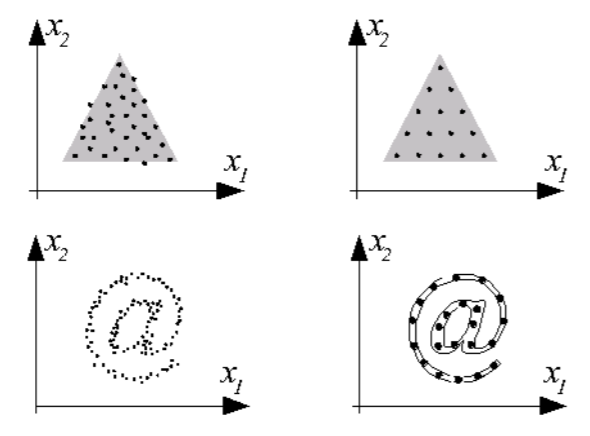
\includegraphics[scale=0.5]{somNet.png}
\caption{Схема сети с самоорганизацией на основе конкуренции}
\label{img:somNetr}
\end{figure}



\subsection{Алгоритм Кохонена}

В нейронных сетях, предложенных Т. Кохоненом (1982 г.), соседство нейронов
носит чисто топологический характер. В простом случае нейроны
слоя Кохонена образуют одномерную цепочку, при этом каждый нейрон
имеет, в общем случае, двух ближайших соседей (слева и справа).
В более сложном случае нейроны Кохонена образуют двумерную сетку
с четырьмя соседями у каждого нейрона (слева, справа, сверху, снизу).
В еще более сложном случае сетка гексагональна — у каждого нейрона
шесть соседей на плоскости (по циферблату часов — 2, 4, 6, 8, 10, 12
часов).
Коррекция весов нейронов в ходе обучения выполняется по формуле

\begin{equation}
W _ { i } ^ { k + 1 } = W _ { i } ^ { k } + \eta ^ { k } G ^ { k } \left( i , X ^ { k } \right) \left( X ^ { k } - W _ { i } ^ { k } \right),
\end{equation}


где функция соседства $G ^ { k } \left( i , X ^ { k } \right)$ определяется, как правило, формулой Гаусса в вид

\begin{equation}
G ^ { k } \left( i , X ^ { k } \right) = \exp \left( - \frac { d ^ { 2 } \left( i , X ^ { k } \right) } { 2 \left( \sigma ^ { k } \right) ^ { 2 } } \right),
\end{equation}

где $d \left( i , X ^ { k } \right)$ ---  расстояние от $i$-ого нейрона до нейрона–победителя с индексом $w_k$ в $k$-ом цикле обучения. При этом $d \left( w ^ { k } , X ^ { k } \right) = 0 , d \left( i , X ^ { k } \right) = 1$ для всех ближайших соседей $w_k$, $d(i, X^k) = 2$ для всех «внешних» ближайших соседей ближайших соседей нейрона победителя с индексом $w^k$ и так далее.

Как обычно, коэффициент обучения $\eta^k$ и параметр ширины функции
Гаусса $\sigma^k$ уменьшаются в ходе обучения (с ростом $k$). В результате обучения слоя Кохонена по такому алгоритму топологически
соседние нейроны становятся типичными представителями кластеров обучающих данных, соседствующих в многомерном пространстве.
В этом достоинство сетей Кохонена, называемых также картами Кохонена, — наглядность в представлении (путем одномерной или двумерной
визуализации) многомерных данных.

Очевидным практическим приложением сетей с самоорганизацией является
сжатие (с потерями) данных, в частности, покадровое сжатие изображений.
Но мы воспользуемся ей для других целей.
Важным свойством сетей с самоорганизацией на основе конкуренции
является способность к кластеризации данных и их распознаванию. Это
обеспечивает их широкое применение для решения задач диагностики,
например, неисправностей оборудовани


\subsection{Алгоритм нейронного газа}
В алгоритме нейронного газа адаптация весов происходит по формуле:
\begin{equation}\label{equ:weightCalc}
    W _ { i } ^ { k + 1 } = W _ { i } ^ { k } + \eta ^ { k } G ^ { k } \left( i , X ^ { k } \right) \left( X ^ { k } - W _ { i } ^ { k } \right),
\end{equation}
В каждом цикле обучения все нейроны сортируются в последовательности возрастания расстояния $d(w^k, X^k)$
\begin{equation}\label{equ:compareLenght}
    d _ { 0 } < d _ { 1 } < \ldots < d _ { j } < \ldots < d _ { M - 1 },
\end{equation}
где $j=m(i)$ — номер i-ого нейрона в последовательности. Для нейрона-победителя $m(i)=0$.

Значение функции соседства i-ого нейрона $G^k(i,X^k)$ определяется следующим выражением:
\begin{equation}\label{equ:neightbourFunc}
G ^ { k } \left( i , \mathbf { X } ^ { k } \right) = \exp \left( - \frac { m ( i ) } { \sigma ^ { k } } \right),
\end{equation}
где $\sigma ^k$ определяет уровень соседства и является величиной, уменьшающейся по ходу обучения. При $\sigma ^k$, стремящемся к 0, алгоритм превращается в алгоритм WTA. Для достижения хороших результатов самоорганизации сети обучение должно начинаться с большого значения $\sigma ^k$, которое с течением времени обучения уменьшается до 0. Для такого уменьшения $\sigma ^k$ предлагается использовать выражение:
\begin{equation}\label{equ:sigma}
    \sigma ^ { k } = \sigma ^ { \max } \cdot \left( \frac { \sigma ^ { \min } } { \sigma ^ { \max } } \right) ^ { \frac { k } { k _ { \max } } },
\end{equation}
где $k_max$ — максимальное заданное количество циклов обучения.

Коэффициент обучения $\eta_i^k$ тоже может уменьшаться с течением времени обучения, это уменьшение может быть линейным от $\eta_max$ в первом цикле до $\eta_min$ в цикле $k_max$, так и показательно в соответствии с формулой:
\begin{equation}\label{equ:eta}
    \eta ^ { k } = \eta _ { \max } \cdot \left( \frac { \eta _ { \max } } { \eta \max } \right) ^ { \frac { k } { k _ { \max } } }.
\end{equation}


\subsection{Реализация}

При поступлении очередной порции данных на вход нейронной сети в рамках каждой эпохи обучения, просходит подсчет весов по формуле \ref{equ:weightCalc}. Но перед этим необходимо определит евклидово расстояние между значениями вектора весов и значениями вектора входных значений, а так же величину функции соседства. В отличие от алгоритма Кохенена, где соседство нейронов определяется близостью их порядкового номера относительно победителя, в алгоритме нейронного газа соседство определяется величиной расстояния до победителя. То есть необходимо для каждого нейрона сначала посчитать расстояние до входных значений по формуле \ref{equ:euclid}, а затем отсортировать в порядке увеличенич значения расстояния (\ref{equ:compareLenght}). Таким образом, первый элемент $d(0)$ в отсортированном массиве расстояний - победитель. Далее нам надо получить индекс нейрона, которому принадлежит это значение расстояния. При расчете функции соседсва для i-го нейрона по формуле \ref{equ:neightbourFunc} мы используем этот индекс нейрона-победителя. Таким образом, нейрон, расположившийся ближе к победителю, значительнее откорректирует свои веса, что нельзя сказать про самый последний, дальний нейрон.

\begin{equation}\label{equ:euclid}
    d \left( X , W _ { i } \right) = \left\| X - W _ { i } \right\| = \sqrt { \sum _ { j = 1 } ^ { N } \left( x _ { j } - w _ { i j } \right) ^ { 2 } }
\end{equation}

Стоит сказать о двух параметрах:
\begin{itemize}
    \item Коэффециент обучения $\eta^k$, где k - номер цикла обучения
    \item Коэффециент соседства $\sigma^k$, где k - номер цикла обучения
\end{itemize}

По мере увеличения времени(итераций), значения коэффициентов $\eta ^ { k }$ и $\sigma ^ { k }$ должны уменьшаться. Для их расчета используются формулы \ref{equ:eta} и \ref{equ:sigma} соответсвенно. Изменяя значение параметра $\eta_{min}$ мы меняем скорость уменьшения коэффециента обучения, $\eta = 0 ... 1$. Величина $\sigma$ может принимать произвольные значения.


Проблема мертвых нейронов на начальном этапе обучения решается путем введения потенциалов (см. раздел \ref{seq:deadNeurons}). 
Минимальный потенциал принимается равным $\pi_{min} = 0.75$ и присваивается изначально всем нейронам.



\subsection{Обучение}
Выборка, на которой происходит обучение, и первоначальное расположение 16-ти нейронов показаны на рис. \ref{img:startpos}.

\begin{figure}[H]
\centering
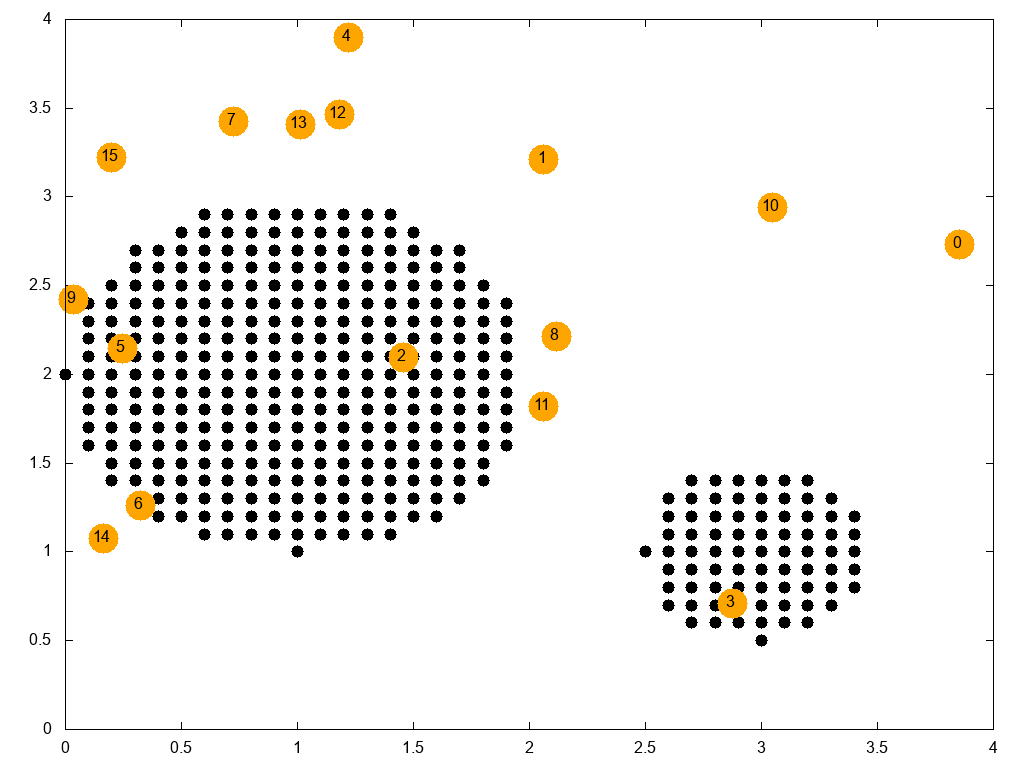
\includegraphics[scale=0.4]{netstartpos.png}
\caption{Обучающая выборка и расположение весов при инициализации}
\label{img:startpos}
\end{figure}

Веса разыграны по равномерному распределению вдоль каждой координатной оси в диапазоне от 0 до 4.

Для того, чтобы дать каждому нейрону возможность проявить себя и ликвидировать мертвые нейроны, произведено $M = 32$ итерации предварительного обучения. При этом использовались слудующие значения коэффециентов:

Значения параметров:
\begin{equation}
	\begin{aligned}
	 &	\sigma_{min} = 0.5,  \\ 
	 &	\sigma_{max} = 2.1, \\	
	 &	\eta_{min} = 0.5,  \\ 
	 &	\eta_{max} = 1, \\
	\end{aligned}
\end{equation} 

В результате, нейроны расположились следующим образом:

\begin{figure}[H]
\centering
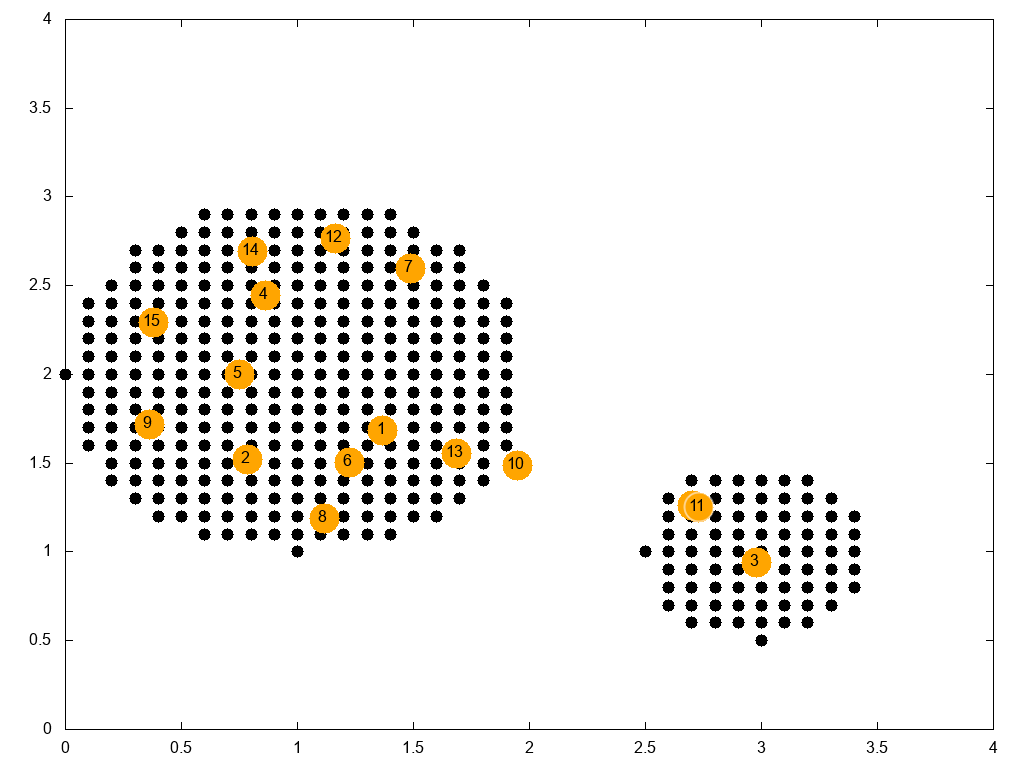
\includegraphics[scale=0.4]{netafterPreTrain.png}
\caption{Расположение нейронов после предварительного обучения ("оживления")}
\label{img:afterPreTrain}
\end{figure}

Для полноценного обучения, при котором больше не происходит изменения потенциалов нейронов, произведен обход входных данных в 10 эпох. Завершение работы алгоритма происходит при окончании всех эпох обучения, без учета минимизации величины ошибки квантования.
Параметры при этом заданы следующие:

\begin{equation}
	\begin{aligned}
	 &	\sigma_{min} = 0.01,  \\ 
	 &	\sigma_{max} = 1., \\	
	 &	\eta_{min} = 0.001,  \\ 
	 &	\eta_{max} = 0.5, \\
	\end{aligned}
\end{equation}

Результирующее распределение нейронов:

\begin{figure}[H]
\centering
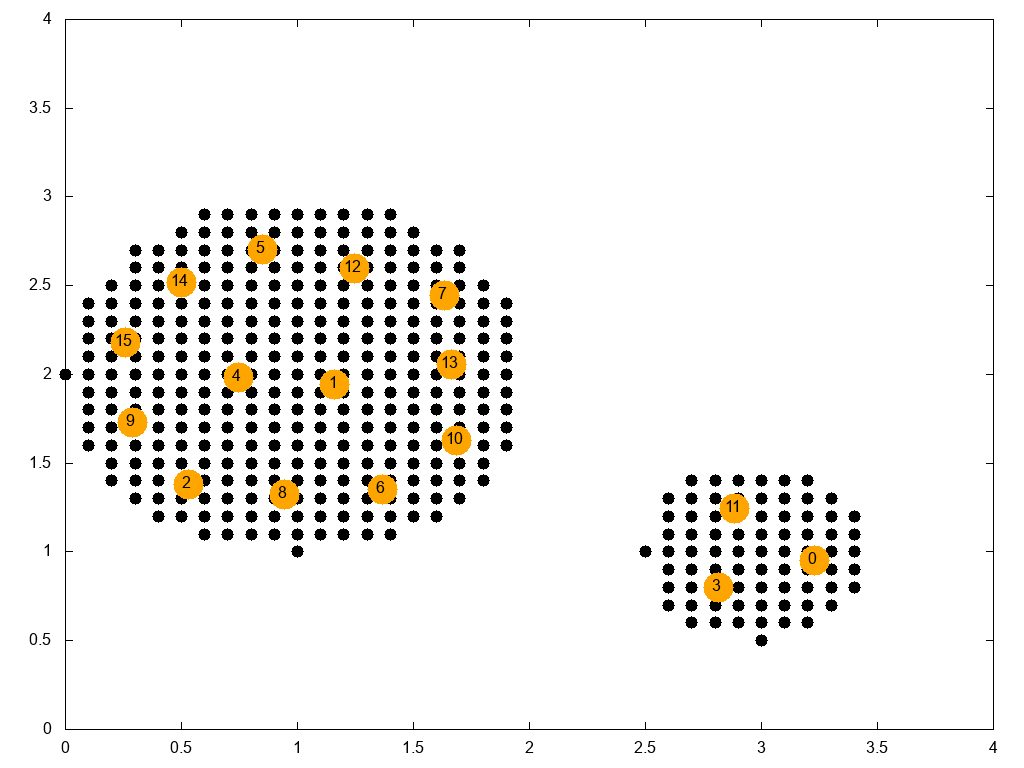
\includegraphics[scale=0.4]{netfinal.png}
\caption{Расположение нейронов после предварительного обучения ("оживления")}
\label{img:finalpos}
\end{figure}



\subsection{Вывод}

На рис. \ref{img:finalpos} видно, что в результате обучения нейроны расположились равномерно по обучающей выборке.

При предварительном обучении исходные параметры $\sigma_{min}$, $\sigma_{max}$, $\eta_{min}$, $\eta_{max}$ следует подбирать таким образом, чтобы за небольшое количество итераций "оживить все нейроны". В случае данной лабораторной работы, при установленный зачениях $\sigma_{min}$, $\sigma_{max}$, $\eta_{min}$, $\eta_{max}$ оживить все 16 нейронов удалось за 32 цикла обучения. Изменяя значения этих коэффециентов можно добиться и более хороших результатов.

В основном цикле обучения использовалась другая конфигурация весов, поэтому значения параметров $\sigma_{max} = 1.1 .. 0.6 $,  $\sigma_{min} = 0.01 .. 0.001$, $\eta_{max} = 0.6 .. 0.3$, $\eta_{min} = 0.001 .. 0.0001$ значительно меньше, по сравнению с предварительным этапом.

\subsection{Код программы}
Файл main.cpp.
\begin{verbatim}
     1	#include "NetSOM.h"
     2	#include <algorithm>
     3	#include <cmath>
     4	#include <random>
     5	
     6	void GenerateSphere(
     7	        std::vector<std::vector<double>> *points,
     8	        double x, double y, 
     9	        double r, double step)
    10	{
    11	    x = (x < 0) ? -x : x;
    12	    y = (y < 0) ? -y : y;
    13	
    14	    for (double xx = -x - r; xx <= x + r; xx += step) {
    15	        for (double yy = -y - r; yy <= y + r; yy += step) {
    16	            if (pow(xx - x, 2) + pow(yy - y, 2) <= pow(r, 2)){ 
    17	                std::vector<double> v(2);
    18	                v[0] = xx;
    19	                v[1] = yy;
    20	                points->emplace_back(std::move(v));
    21	            }
    22	        }
    23	    }
    24	}
    25	
    26	// ---------------------------------------------------------------------
------------------
    27	void SaveTrainSetToFile(std::ostream &output, const std::vector<std::vec
tor<double>> &points) {
    28	    for (size_t iPoint = 0; iPoint < points.size(); ++iPoint) {
    29	        for (size_t iCoord = 0; iCoord < points[iPoint].size(); ++iCoord
)
    30	            output << points[iPoint][iCoord] << "\t";
    31	        output << std::endl;
    32	    }
    33	}
    34	
    35	int main() {
    36	    std::vector<std::vector<double>> trainSet;
    37	    GenerateSphere (&trainSet, 1., 2., 1., 0.1);
    38	    GenerateSphere (&trainSet, 3., 1., 0.5, 0.1);
    39	    //std::random_shuffle(trainSet.begin(), trainSet.end());
    40	
    41	    Net  net;
    42	    Net::NetConfig netConf;
    43	
    44	    netConf.neurons  = 16;
    45	    netConf.inVecDim = 2;
    46	    netConf.trainEpochs = 10.;
    47	    netConf.preTrainIterations = 32;
    48	    netConf.minPotential = 0.75;
    49	    netConf.deltaMinFuncEps = 1e-3;
    50	
    51	    netConf.sigmaInitPreTrain = 2.1;
    52	    netConf.sigmaInitPreTrainMin = 0.5;
    53	    netConf.etaInitPreTrain = 1.;
    54	    netConf.etaInitPreTrainMin = 0.5;
    55	
    56	    netConf.sigmaInit = 1.;
    57	    netConf.sigmaInitMin = 1e-1;
    58	    netConf.etaInit = 0.5;
    59	    netConf.etaInitMin = 1e-3;
    60	    netConf.weightLowBound   = 0.;
    61	    netConf.weightUpperBound = 4.;
    62	
    63	    netConf.weightFileName = std::string("weight.data");
    64	
    65	    net.Init(netConf);
    66	
    67	    std::ofstream trainSetFile("train.data", std::ios::trunc);
    68	    std::ofstream weightFile(netConf.weightFileName, std::ios::trunc);
    69	    std::ofstream gnuplotFile("plot.txt", std::ios::trunc);
    70	
    71	    SaveTrainSetToFile(trainSetFile, trainSet);
    72	    //exit(1);
    73	    net.TrainGas(trainSet, weightFile);
    74	    net.CreateGnuplotAnimation(gnuplotFile);
    75	    std::cerr << "End of training " << std::endl;
    76	}

\end{verbatim}

Файл Net.cpp
\begin{verbatim}
     1	#include "Net.h"
     2	#include <iomanip>
     3	#include <random>
     4	#include <algorithm>
     5	#include <limits>
     6	#include <fstream>
     7	#include <unistd.h>
     8	
     9	void Net::Init(const NetConfig &conf) {
    10	    config = conf;
    11	    weights.resize(config.neurons * config.inVecDim);
    12	    potential.resize(config.neurons, config.minPotential);
    13	    neuronsNeighbourSequence.resize(config.neurons, 0);
    14	    victory.resize(config.neurons, 0);
    15	    RandomWeights();
    16	}
    17	bool compare(const std::pair<double, double>&i, const std::pair<double, 
double>&j){ 
    18	    return i.first < j.first; 
    19	}
    20	
    21	void Net::RandomWeights() {
    22	    std::random_device randomizer;
    23	    std::mt19937 randGen(randomizer());
    24	    std::uniform_real_distribution<> dist(config.weightLowBound, 
    25	                                          config.weightUpperBound);
    26	    double weightNorm;
    27	    double weight = 0.0;
    28	    for (size_t iNeuron = 0; iNeuron < config.neurons; ++iNeuron) {
    29	        for (size_t iWeight = 0; iWeight < config.inVecDim; ++iWeight) {
    30	            weight = dist(randGen);
    31	            std::cerr << weight << std::endl;
    32	            weights[iWeight + iNeuron * config.inVecDim] = weight;
    33	        }
    34	    }
    35	}
    36	
    37	size_t Net::DetectWinnerGas(const std::vector<double> &inVec) {
    38	
    39	    std::vector<std::pair<double, int>>  distancesToInput (config.neuron
s, std::pair<double, int> (0.0, 0));
    40	
    41	    // calculate distance for each neuron
    42	    for (size_t iNeuron = 0; iNeuron < config.neurons; ++iNeuron) {
    43	        for (size_t iWeight = 0; iWeight < config.inVecDim; ++iWeight) 
    44	            distancesToInput[iNeuron].first += pow(inVec[iWeight] - weig
hts[iWeight + iNeuron * config.inVecDim], 2);
    45	
    46	        if (potential[iNeuron] < config.minPotential)
    47	            distancesToInput[iNeuron].first = std::numeric_limits<double
>::max();
    48	        else 
    49	            distancesToInput[iNeuron].first = potential[iNeuron] * sqrt(
distancesToInput[iNeuron].first);
    50	
    51	        distancesToInput[iNeuron].second = iNeuron;
    52	    }
    53	
    54	    std::sort(distancesToInput.begin(), distancesToInput.end(), compare)
;
    55	
    56	    std::cout << "+SORTED distances" << std::endl;
    57	    for (size_t i = 0; i < distancesToInput.size(); ++i)
    58	      std::cout << distancesToInput[i].first << " " << distancesToInput[
i].second << std::endl;
    59	
    60	    std::cout << "Neightbours sequence is";
    61	    for (size_t i = 0; i < distancesToInput.size(); ++i){
    62	      neuronsNeighbourSequence[i] = distancesToInput[i].second;
    63	      std::cout << ' ' << neuronsNeighbourSequence[i];
    64	    }
    65	    std::cout << std::endl;
    66	
    67	    size_t winnerInd = distancesToInput[0].second;
    68	    std::cout << "winnerInd is " << winnerInd << std::endl;
    69	
    70	    victory[winnerInd] ++;
    71	    std::cout << "Счетчик побед: ";
    72	    for (int &a: victory)
    73	      std::cout << ' ' << a;
    74	    std::cout << '\n';
    75	
    76	    
    77	    return winnerInd;
    78	}
    79	
    80	size_t Net::GetIndexInNeuronsNeighbourSequence(size_t neuronNumber){
    81	    std::vector<int>::iterator it = std::find(neuronsNeighbourSequence.b
egin(), 
    82	                                              neuronsNeighbourSequence.e
nd(), 
    83	                                              neuronNumber);
    84	    /*if ! (it != neuronsNeighbourSequence.end())
    85	        throw std::string("Net::GetIndexInNeuronsNeighbourSequence --> E
lement Not Found!");*/
    86	
    87	    // Get index of element from iterator
    88	    int index = std::distance(neuronsNeighbourSequence.begin(), it);
    89	    return index;
    90	}
    91	
    92	void Net::AdjustWeightsKohen(size_t winnerInd, const std::vector<double>
 &inVec) {
    93	    for (size_t iNeuron = 0; iNeuron < config.neurons; ++iNeuron) {
    94	        for (size_t iWeight = 0; iWeight < config.inVecDim; ++iWeight) {
    95		          double d = fabs(iNeuron - winnerInd);
    96		          double neigbourCoeff = exp(-pow(d / sigma, 2) / 2);
    97	            weights[iWeight + iNeuron * config.inVecDim] += eta * neigbo
urCoeff 
    98	              * (inVec[iWeight] - weights[iWeight + iNeuron * config.inV
ecDim]);
    99	        }
   100	    }
   101	}
   102	
   103	void Net::AdjustWeightsGas(const std::vector<double> &inVec) {
   104	    for (size_t iNeuron = 0; iNeuron < config.neurons; ++iNeuron) {
   105	        int m = GetIndexInNeuronsNeighbourSequence(iNeuron);
   106	        double neigbourCoeff = exp(- m / sigma);
   107	        for (size_t iWeight = 0; iWeight < config.inVecDim; ++iWeight) {
   108	            weights[iWeight + iNeuron * config.inVecDim] += eta * neigbo
urCoeff 
   109	              * (inVec[iWeight] - weights[iWeight + iNeuron * config.inV
ecDim]);
   110	        }
   111	    }
   112	}
   113	
   114	void Net::AdjustPotential(size_t winnerInd) {
   115	    std::cout << std::endl << "Список потенциалов:" << 
std::endl;
   116	    for (size_t iPotential = 0; iPotential < potential.size(); iPotentia
l++) {
   117	        (iPotential == winnerInd) ? potential[iPotential] -= config.minP
otential
   118	                                  : potential[iPotential] += 1. / config
.neurons;
   119	        std::cout << potential[iPotential] << std::endl;
   120	    }
   121	    std::cout << std::endl;
   122	}
   123	
   124	void Net::TrainGas(std::vector<std::vector<double>> &trainSet,
   125	                     std::ostream &outputLabels) 
   126	{
   127	    size_t winnerInd;
   128	    double maxT;
   129	    // предварительная подготовка весов
   130	    std::random_shuffle(trainSet.begin(), trainSet.end());
   131	    PrintWeightsToFile(outputLabels, 16);
   132	
   133	    maxT = config.preTrainIterations - 1; 
   134	    for (size_t iVec = 0; iVec < config.preTrainIterations; ++iVec) {
   135	        double time = iVec + 1;  
   136	        sigma = config.sigmaInitPreTrain 
   137	              * pow(config.sigmaInitPreTrainMin / config.sigmaInitPreTra
in, time / maxT);
   138	        eta   = config.etaInitPreTrain   
   139	              * pow(config.etaInitPreTrainMin   / config.etaInitPreTrain
  , time / maxT);
   140	        winnerInd = DetectWinnerGas(trainSet[iVec]);
   141	        AdjustPotential(winnerInd);
   142	        AdjustWeightsGas(trainSet[iVec]);
   143	        PrintWeightsToFile(outputLabels, 16);
   144	    }
   145	    sleep(5);
   146	
   147	    for (int iPot = 0; iPot < potential.size(); iPot++) {
   148	        potential[iPot] = 1.;
   149	    }
   150	    maxT = config.trainEpochs * trainSet.size(); // k max = maxT, k = ti
me
   151	    double time = 0.;
   152	    for (size_t iEpoch = 0; iEpoch < config.trainEpochs; ++iEpoch) {
   153	        std::random_shuffle(trainSet.begin(), trainSet.end());
   154	        for (size_t iVec = 0; iVec < trainSet.size(); ++iVec) {
   155	            time++;
   156	            sigma = config.sigmaInit * pow(config.sigmaInitMin / config.
sigmaInit, time / maxT);
   157	            eta   = config.etaInit   * pow(config.etaInitMin   / config.
etaInit  , time / maxT);
   158	            winnerInd = DetectWinnerGas(trainSet[iVec]);
   159	            //AdjustPotential(winnerInd);
   160	            AdjustWeightsGas(trainSet[iVec]);
   161	            PrintWeightsToFile(outputLabels, 16);
   162	        }
   163	    }
   164	}
   165	
   166	void Net::PrintWeightsToFile(std::ostream &output, int precision) {
   167	    for (size_t iWeight = 0; iWeight < weights.size(); ++iWeight) {
   168	        output << std::setprecision(precision) << weights[iWeight] << "\
t";
   169	        if (iWeight % 2) {
   170	            output << iWeight / config.inVecDim << "\t";
   171	        }
   172	    }
   173	    output << std::endl << std::endl << std::endl;
   174	}
   175	
   176	void Net::CreateGnuplotAnimation(std::ofstream &stream) {
   177	    stream << " set terminal gif size 1024, 768 animate delay 0.001 loop
 -1 "<< std::endl
   178	              << " set output 'train.gif' "<< std::endl
   179	              << " set xrange [0:4] "<< std::endl
   180	              << " set yrange [0:4] "<< std::endl
   181	              << " unset key "<< std::endl              
   182	              << " stats \'" << config.weightFileName << "\' nooutput  "
<< std::endl
   183	              << " do for [i=1:int(STATS_blocks)-1] { "<< std::endl
   184	              << "     plot \"train.data\" index 0 using 1:2 pt 7 ps 2 l
c rgb \'black\',\\"<< std::endl;
   185	    for (size_t iNeuron = 0; iNeuron < config.neurons - 1; iNeuron++) {
   186	        stream << "      \"" << config.weightFileName <<"\" index(i-1) u
sing " 
   187	               <<  (iNeuron+1)*3 - 2 << ":" << (iNeuron+1)*3 - 1
   188	               << "  pt 7 ps 5 lc rgb \'orange\',\\"<< std::endl;
   189	        stream << "      \"" << config.weightFileName <<"\" index(i-1) u
sing " 
   190	               <<  (iNeuron+1)*3 - 2 << ":" << (iNeuron+1)*3 - 1 << ":" 
<< (iNeuron+1)*3
   191	               << "  with labels,\\"<< std::endl;
   192	    }
   193	    stream << "      \"" << config.weightFileName <<"\" index(i-1) using
 " 
   194	           <<  (config.neurons)*3 - 2 << ":" << (config.neurons)*3 - 1
   195	           << "  pt 7 ps 5 lc rgb \'orange\',\\"<< std::endl;
   196	    stream << "      \"" << config.weightFileName <<"\" index(i-1) using
 " 
   197	           <<  (config.neurons)*3 - 2 << ":" << (config.neurons)*3 - 1 <
< ":" << (config.neurons)*3
   198	           << "  with labels\\"<< std::endl;
   199	    stream << "}" << std::endl;
   200	
   201	    std::ofstream file;
   202	    file.open("finalpos.txt", std::ios::trunc);
   203	    file << " set terminal gif size 1024, 768 animate delay 0.001 loop -
1 "<< std::endl
   204	              << " set output 'final.gif' "<< std::endl
   205	              << " set xrange [0:4] "<< std::endl
   206	              << " set yrange [0:4] "<< std::endl
   207	              << " unset key "<< std::endl              
   208	              << " stats 'weight.data' nooutput  "<< std::endl
   209	              << " do for [i=int(STATS_blocks)-1:int(STATS_blocks)-1] { 
"<< std::endl
   210	              << "     plot \"train.data\" index 0 using 1:2 pt 7 ps 2 l
c rgb \'black\',\\"<< std::endl;
   211	    for (size_t iNeuron = 0; iNeuron < config.neurons - 1; iNeuron++) {
   212	        file << "      \"" << config.weightFileName <<"\" index(i-1) usi
ng " 
   213	               <<  (iNeuron+1)*3 - 2 << ":" << (iNeuron+1)*3 - 1
   214	               << "  pt 7 ps 5 lc rgb \'orange\',\\"<< std::endl;
   215	        file << "      \"" << config.weightFileName <<"\" index(i-1) usi
ng " 
   216	               <<  (iNeuron+1)*3 - 2 << ":" << (iNeuron+1)*3 - 1 << ":" 
<< (iNeuron+1)*3
   217	               << "  with labels,\\"<< std::endl;
   218	    }
   219	    file << "      \"" << config.weightFileName <<"\" index(i-1) using "
 
   220	           <<  (config.neurons)*3 - 2 << ":" << (config.neurons)*3 - 1
   221	           << "  pt 7 ps 5 lc rgb \'orange\',\\"<< std::endl;
   222	    file << "      \"" << config.weightFileName <<"\" index(i-1) using "
 
   223	           <<  (config.neurons)*3 - 2 << ":" << (config.neurons)*3 - 1 <
< ":" << (config.neurons)*3
   224	           << "  with labels\\"<< std::endl;
   225	    file << "}" << std::endl;
   226	
   227	    std::ofstream fileStart;
   228	    fileStart.open("startpos.txt", std::ios::trunc);
   229	    fileStart << " set terminal gif size 1024, 768 animate delay 0.001 l
oop -1 "<< std::endl
   230	              << " set output 'startpos.gif' "<< std::endl
   231	              << " set xrange [0:4] "<< std::endl
   232	              << " set yrange [0:4] "<< std::endl
   233	              << " unset key "<< std::endl              
   234	              << " stats 'weight.data' nooutput  "<< std::endl
   235	              << " do for [i=1:1] { "<< std::endl
   236	              << "     plot \"train.data\" index 0 using 1:2 pt 7 ps 2 l
c rgb \'black\',\\"<< std::endl;
   237	    for (size_t iNeuron = 0; iNeuron < config.neurons - 1; iNeuron++) {
   238	        fileStart << "      \"" << config.weightFileName <<"\" index(i-1
) using " 
   239	               <<  (iNeuron+1)*3 - 2 << ":" << (iNeuron+1)*3 - 1
   240	               << "  pt 7 ps 5 lc rgb \'orange\',\\"<< std::endl;
   241	        fileStart << "      \"" << config.weightFileName <<"\" index(i-1
) using " 
   242	               <<  (iNeuron+1)*3 - 2 << ":" << (iNeuron+1)*3 - 1 << ":" 
<< (iNeuron+1)*3
   243	               << "  with labels,\\"<< std::endl;
   244	    }
   245	    fileStart << "      \"" << config.weightFileName <<"\" index(i-1) us
ing " 
   246	           <<  (config.neurons)*3 - 2 << ":" << (config.neurons)*3 - 1
   247	           << "  pt 7 ps 5 lc rgb \'orange\',\\"<< std::endl;
   248	    fileStart << "      \"" << config.weightFileName <<"\" index(i-1) us
ing " 
   249	           <<  (config.neurons)*3 - 2 << ":" << (config.neurons)*3 - 1 <
< ":" << (config.neurons)*3
   250	           << "  with labels\\"<< std::endl;
   251	    fileStart << "}" << std::endl;
   252	
   253	    std::ofstream filePreTrain;
   254	    filePreTrain.open("afterPreTrain.txt", std::ios::trunc);
   255	    int outIter = config.preTrainIterations;
   256	    filePreTrain << " set terminal gif size 1024, 768 animate delay 0.00
1 loop -1 "<< std::endl
   257	              << " set output 'afterPreTrain.gif' "<< std::endl
   258	              << " set xrange [0:4] "<< std::endl
   259	              << " set yrange [0:4] "<< std::endl
   260	              << " unset key "<< std::endl              
   261	              << " stats 'weight.data' nooutput  "<< std::endl
   262	              << " do for [i=" << outIter << ":" << outIter <<"] { "<< s
td::endl
   263	              << "     plot \"train.data\" index 0 using 1:2 pt 7 ps 2 l
c rgb \'black\',\\"<< std::endl;
   264	    for (size_t iNeuron = 0; iNeuron < config.neurons - 1; iNeuron++) {
   265	        filePreTrain << "      \"" << config.weightFileName <<"\" index(
i-1) using " 
   266	               <<  (iNeuron+1)*3 - 2 << ":" << (iNeuron+1)*3 - 1
   267	               << "  pt 7 ps 5 lc rgb \'orange\',\\"<< std::endl;
   268	        filePreTrain << "      \"" << config.weightFileName <<"\" index(
i-1) using " 
   269	               <<  (iNeuron+1)*3 - 2 << ":" << (iNeuron+1)*3 - 1 << ":" 
<< (iNeuron+1)*3
   270	               << "  with labels,\\"<< std::endl;
   271	    }
   272	    filePreTrain << "      \"" << config.weightFileName <<"\" index(i-1)
 using " 
   273	           <<  (config.neurons)*3 - 2 << ":" << (config.neurons)*3 - 1
   274	           << "  pt 7 ps 5 lc rgb \'orange\',\\"<< std::endl;
   275	    filePreTrain << "      \"" << config.weightFileName <<"\" index(i-1)
 using " 
   276	           <<  (config.neurons)*3 - 2 << ":" << (config.neurons)*3 - 1 <
< ":" << (config.neurons)*3
   277	           << "  with labels\\"<< std::endl;
   278	    filePreTrain << "}" << std::endl;
   279	
   280	}
\end{verbatim}

Файл Net.h
\begin{verbatim}
     1	#include <vector>
     2	#include <iostream>
     3	#include <fstream>
     4	using size_t = std::size_t;
     5	
     6	class Net {
     7	public:
     8	    struct NetConfig {
     9	        size_t neurons;
    10	        size_t inVecDim;
    11	        int    trainEpochs;
    12	        int    preTrainIterations;
    13	        double minPotential;
    14	        double deltaMinFuncEps;
    15	        
    16	        double sigmaInitPreTrain;
    17	        double etaInitPreTrain;
    18	        double sigmaInitPreTrainMin;
    19	        double etaInitPreTrainMin;
    20	        
    21	        double sigmaInit;
    22	        double etaInit;
    23	        double sigmaInitMin;
    24	        double etaInitMin;
    25	
    26	        double weightLowBound;
    27	        double weightUpperBound;
    28	
    29	        std::string weightFileName;
    30	    };
    31	
    32	    void Init(const NetConfig &conf);
    33	    void TrainKohen(std::vector<std::vector<double>> &trainSet, std::ost
ream &outputLabels);
    34	    void TrainGas(std::vector<std::vector<double>> &trainSet, std::ostre
am &outputLabels);
    35	    void PrintWeightsToFile(std::ostream &output, int precision);
    36	    void CreateGnuplotAnimation(std::ofstream &stream);
    37	    size_t DetectWinnerKohen(const std::vector<double> &inVec);
    38	    size_t DetectWinnerGas(const std::vector<double> &inVec);
    39	
    40	private:
    41	    NetConfig config;
    42	    std::vector<double>   weights;
    43	    std::vector<double>   potential;
    44	    std::vector<int>      neuronsNeighbourSequence; // for DetectWinnerK
ohen
    45	    std::vector<int>      victory;
    46	    double sigma;
    47	    double eta;
    48	    void RandomWeights();
    49	    void AdjustWeightsKohen(size_t winnerInd, const std::vector<double> 
&inVec);
    50	    void AdjustWeightsGas(const std::vector<double> &inVec);
    51	    void AdjustPotential(size_t winnerInd);
    52	    void AdjustPotentialInverted(size_t winnerInd);
    53	    size_t GetIndexInNeuronsNeighbourSequence(size_t neuronNumber);
    54	};

\end{verbatim}

%\input{RefProject-Algoritm}% это описание алгоритмов
%\input{RefProject-Finish}% заключение
%\input{RefProject-App}% приложение

\end{document}
